%--------------------------------------------------------------------%
%
% Berkas utama templat LaTeX.
%
% author Petra Barus, Peb Ruswono Aryan, Faris Rizki Ekananda
%
%--------------------------------------------------------------------%
%
% Berkas ini berisi struktur utama dokumen LaTeX yang akan dibuat.
%
%--------------------------------------------------------------------%

\documentclass[bahasa, 12pt, a4paper, onecolumn, oneside, final]{report}

%-------------------------------------------------------------------%
%
% Konfigurasi dokumen LaTeX untuk laporan tesis IF ITB
%
% @author Petra Novandi
%
%-------------------------------------------------------------------%
%
% Berkas asli berasal dari Steven Lolong
%
%-------------------------------------------------------------------%

% Ukuran kertas
\special{papersize=210mm,297mm}

% Setting margin
\usepackage[top=3cm,bottom=3cm,left=4cm,right=3cm]{geometry}

\usepackage{mathptmx}

% Judul bahasa Indonesia
\usepackage[bahasa]{babel}

% Format citation
\usepackage[style=apa,backend=biber]{biblatex}

\usepackage[utf8]{inputenc}
\usepackage{graphicx}
\usepackage{titling}
\usepackage{blindtext}
\usepackage{sectsty}
\usepackage{chngcntr}
\usepackage{etoolbox}
\usepackage{hyperref}       % Package untuk link di daftar isi. Ubah jadi \usepackage[hidelinks]{hyperref} apabila ingin menghilangkan kotak merah disekitar link
\usepackage{titlesec}       % Package Format judul
\usepackage{titletoc}       % Package Format judul di toc
\usepackage{tocbibind}      % Package untuk masukkan toc, lot, lof ke Daftar Isi
\usepackage{scrwfile}       % Package untuk membuat Daftar Lampiran dari toc
\usepackage{parskip}
\usepackage{afterpage}
\usepackage{relsize}
\usepackage{pgfgantt}       % Package untuk membuat Gantt Chart
\usepackage{lscape}         % Package untuk membuat landscape

\graphicspath{{resources/}}   % letak direktori penyimpanan gambar

% Setting daftar lampiran
\newcommand*{\lopname}{DAFTAR LAMPIRAN}
\TOCclone[\lopname]{toc}{atoc}
\addtocontents{atoc}{\protect\value{tocdepth}=-1}
\newcommand\listofappendices{
  \cleardoublepage
  \phantomsection
  \listofatoc
  \addcontentsline{toc}{chapter}{\lopname}
}

\newcommand*\savedtocdepth{}
\AtBeginDocument{%
  \edef\savedtocdepth{\the\value{tocdepth}}%
}

\let\originalappendix\appendix
\renewcommand\appendix{%
  \originalappendix
  \cleardoublepage
  \addtocontents{toc}{\protect\value{tocdepth}=-1}%
  \addtocontents{atoc}{\protect\value{tocdepth}=\savedtocdepth}%

  \titlecontents{chapter}
    [0pt]
    {\bfseries}
    {Lampiran \thecontentslabel.\quad}
    {}
    {\hfill\contentspage}

  \titleformat{\chapter}[block]
    {\bfseries}
    {\chaptertitlename\ \thechapter.\quad}{0pt}
    {\bfseries}
}

% Hilangkan titik pada toc
\makeatletter
\renewcommand{\@dotsep}{10000}
\makeatother

% Setel title pada chapter-chapter di toc, lof, lot
\titlecontents{chapter}
  [0pt]
  {\bfseries}
  {\MakeUppercase{Bab} \thecontentslabel\quad\uppercase}
  {}
  {\hfill\contentspage}
\titlecontents{figure}
  [0pt]
  {}
  {Gambar \thecontentslabel.\quad}
  {}
  {\hfill\contentspage}
\titlecontents{table}
  [0pt]
  {}
  {Tabel \thecontentslabel.\quad}
  {}
  {\hfill\contentspage}

% Masukin Daftar Pustaka ke toc
\let\originalprintbibliography\printbibliography
\renewcommand\printbibliography{%
  \phantomsection
  \cleardoublepage
  \originalprintbibliography
  \addcontentsline{toc}{chapter}{\bibname}
}

% Line satu setengah spasi
\renewcommand{\baselinestretch}{1.5}

% Setting judul
\chapterfont{\centering \Large}
\titleformat{\chapter}[display]
  {\Large\centering\bfseries}
  {\chaptertitlename\ \thechapter}{0pt}
    {\Large\bfseries\uppercase}

% Setting nomor pada subbsubsubbab
\setcounter{secnumdepth}{3}

\makeatletter

\makeatother

% Counter untuk figure dan table.
\counterwithin{figure}{section}
\counterwithin{table}{section}

% Define blank page
\newcommand*{\blankpage}{\afterpage{\null\newpage}}

% Remove Hypenation
\hyphenpenalty=10000
\exhyphenpenalty=10000
\sloppy % Makes TeX obey margins by stretching inter word spaces


\makeatletter

\makeatother

\addbibresource{references.bib}

\begin{document}

% Basic configuration
% date and times
\newcommand{\thedate}{\date{23 Juni 2023}}
\newcommand{\monthyear}{JUNI 2023}

% titles
\newcommand{\capstonetitle}{Pengembangan Sistem Simulasi \textit{Autonomous Tram} dengan Simulator CARLA}
\newcommand{\thetitle}{Implementasi Objek Lokal dan Lingkungan Indonesia untuk Simulasi
Trem Otonom Menggunakan Simulator CARLA}

\title{\thetitle}

\newcommand{\subtitle}{
    \bfseries \Large
    Laporan Tugas Akhir - Capstone

    \capstonetitle
}

% identity
\newcommand{\authorname}{Jeane Mikha Erwansyah}
\newcommand{\authornim}{13519116}
\author{
    \authorname \\
    NIM : \authornim
}

% \newcommand{\advisoronename}{Achmad Imam Kistijantoro, S.T., M.Sc., Ph.D.}
% \newcommand{\advisoronenip}{197308092006041001}
% \newcommand{\advisortwoname}{Prof. Dr. Ir. Bambang Riyanto Trilaksono}
% \newcommand{\advisortwonip}{196211151987031004}

% advisors
\newcommand{\advisoronename}{Achmad Imam Kistijantoro, Ph.D.}
\newcommand{\advisoronenip}{197308092006041001}
\newcommand{\advisortwoname}{Prof. Dr. Bambang Riyanto Trilaksono}
\newcommand{\advisortwonip}{196211151987031004}
\newcommand{\advisorapproval}{
    \centering
    \normalsize \normalfont
    % commented out because of differences between capstone-team and approval-2
    % Bandung, \thedate \\
    % Mengetahui,

    \vspace{0.5cm}
    \setlength{\tabcolsep}{12pt}
    \begin{tabular}{c@{\hskip 0.5cm}c}
        Pembimbing I,               & Pembimbing II,             \\
                                    &                            \\
                                    &                            \\
                                    &                            \\
                                    &                            \\
        \underline{\advisoronename} & \underline{\advisortwoname} \\
        NIP. \advisoronenip     & NIP. \advisortwonip     \\
    \end{tabular}
    }

\pagenumbering{roman}
\setcounter{page}{1}

\clearpage
\pagestyle{empty}

\begin{center}
    \smallskip

    \Large \bfseries \MakeUppercase{\thetitle}
    \vfill

    \subtitle
    \vfill

    \large Disusun sebagai syarat kelulusan tingkat sarjana
    \vfill

    \large Oleh

    \Large \theauthor

    \vfill
    \begin{figure}[h]
        \centering
        \includegraphics[width=0.15\textwidth]{cover-ganesha.jpg}
    \end{figure}
    \vfill

    \large
    \uppercase{
        Program Studi Teknik Informatika \\
        Sekolah Teknik Elektro \& Informatika \\
        Institut Teknologi Bandung
    }

    \monthyear

\end{center}

\clearpage

\clearpage
\pagestyle{empty}

\begin{center}
    \smallskip

    \Large \bfseries \MakeUppercase{\thetitle}
    \vfill

    \subtitle
    \vfill

    \large Oleh

    \Large \theauthor

    \large Program Studi Teknik Informatika \\

    \normalsize \normalfont
    Sekolah Teknik Elektro dan Informatika \\
    Institut Teknologi Bandung

    \vfill
    \advisorapproval

\end{center}
\clearpage
\clearpage
\pagestyle{empty}

\begin{center}
	\smallskip

	\Large \bfseries \MakeUppercase{
		Lembar Identitas \\
		Tugas Akhir Capstone
	}
	\vspace{0.5cm}

	\raggedright
	\begin{table}[h!]
		\large \bfseries
		\begin{onehalfspace}
		\begin{tabular}{p{0.3\textwidth} p{0.63\textwidth}}
			Judul Proyek TA : & \capstonetitle \\
		\end{tabular}
		\end{onehalfspace}
	\end{table}

	\normalsize \normalfont

	Anggota tim dan pembagian peran:

	\begin{table}[h!]
		\begin{onehalfspace}
		\begingroup
		\def\arraystretch{1.25}
		\begin{tabular}{|p{0.05\textwidth} | p{0.13\textwidth} | p{0.19\textwidth} | p{0.50\textwidth}|}
			\hline
			\textbf{No.} & \textbf{NIM} & \textbf{Nama}         & \textbf{Peran} \\
			\hline
			1.           & 13519116     & Jeane Mikha Erwansyah & \thetitle \\
			\hline
			2.           & 13519164     & Josep Marcello        & Pengembangan Mekanisme Komunikasi \textit{Hardware-in-the-Loop-Simulation} untuk Kendaraan Otonom \\
			\hline
			3.           & 13519188     & Jeremia Axel Bachtera & Pembangunan Modul Pengujian untuk Simulasi Trem Otonom Simulator CARLA \\
			\hline
		\end{tabular}
		\endgroup
		\end{onehalfspace}
	\end{table}

	\vfill
	\begin{center}
		\normalsize \normalfont
		Bandung, \thedate \\
		Mengetahui,
	\end{center}
	\advisorapproval

\end{center}
\clearpage


\pagestyle{plain}

\titleformat*{\section}{\centering\bfseries\Large\MakeUpperCase}
\titlespacing*{\chapter}{0pt}{0pt}{3pc}

\chapter*{Lembar Pernyataan}

Dengan ini saya menyatakan bahwa:

\begin{enumerate}

    \item Pengerjaan dan penulisan Laporan Tugas Akhir ini dilakukan tanpa
    menggunakan bantuan yang tidak dibenarkan.
    \item Segala bentuk kutipan dan acuan terhadap tulisan orang lain yang
    digunakan di dalam penyusunan laporan tugas akhir ini telah dituliskan
    dengan baik dan benar.
    \item Laporan Tugas Akhir ini belum pernah diajukan pada program pendidikan
    di perguruan tinggi mana pun.

\end{enumerate}

Jika terbukti melanggar hal-hal di atas, saya bersedia dikenakan sanksi sesuai
dengan Peraturan Akademik dan Kemahasiswaan Institut Teknologi Bandung bagian
Penegakan Norma Akademik dan Kemahasiswaan khususnya Pasal 2.1 dan Pasal 2.2.
\vspace{15mm}

Bandung, \thedate \\

\vspace{15mm}

\underline{\authorname} \\
NIM \authornim

\clearpage

\clearpage
\chapter*{ABSTRAK}
\addcontentsline{toc}{chapter}{Abstrak}

%taruh abstrak bahasa indonesia di sini
\blindtext
\clearpage
% \clearpage
\chapter*{Abstract}
\addcontentsline{toc}{chapter}{Abstract}

%put your abstract here
\blindtext

\clearpage
\chapter*{Kata Pengantar}
\addcontentsline{toc}{chapter}{KATA PENGANTAR}

Gunakan bagian ini untuk memberikan ucapan terima kasih kepada semua pihak yang
secara langsung atau tidak langsung membantu penyelesaian tugas akhir, termasuk
pemberi beasiswa jika ada. Utamakan untuk memberikan ucapan terima kasih kepada
tim pembimbing tugas akhir dan staf pengajar atau pihak program studi, bahkan
sebelum mengucapkan terima kasih kepada keluarga. Ucapan terima kasih sebaiknya
bukan hanya menyebutkan nama orang saja, tetapi juga memberikan penjelasan
bagaimana bentuk bantuan/dukungan yang diberikan. Gunakan bahasa yang baik dan
sopan serta memberikan kesan yang enak untuk dibaca. Sebagai contoh: “Tidak lupa
saya ucapkan terima kasih kepada teman dekat saya, Tito, yang sejak satu tahun
terakhir ini selalu memberikan semangat dan mengingatkan saya apabila lengah
dalam mengerjakan Tugas Akhir ini. Tito juga banyak membantu mengoreksi format
dan layout tulisan. Apresiasi saya sampaikan kepada pemberi beasiswa, Yayasan
Beasiswa, yang telah memberikan bantuan dana kuliah dan biaya hidup selama dua
tahun. Bantuan dana tersebut sangat membantu saya untuk dapat lebih fokus dalam
menyelesaikan pendidikan saya. ....”. Ucapan permintaan maaf karena
kekurangsempurnaan hasil Tugas Akhir tidak perlu ditulis.

\begin{flushright}
	Bandung, \thedate \\
	\vspace{15mm}

	Penulis
\end{flushright}



% Setting judul toc, lot, lof, bib
\renewcommand{\contentsname}{DAFTAR ISI}
\renewcommand{\listfigurename}{DAFTAR GAMBAR}
\renewcommand{\listtablename}{DAFTAR TABEL}
\renewcommand{\bibname}{DAFTAR PUSTAKA}

% \renewcommand{\cftchapleader}{\cftdot} % for chapters

\tableofcontents
% \listofappendices
\listoffigures
% \listoftables
\chapter*{Daftar Istilah}
\addcontentsline{toc}{chapter}{DAFTAR ISTILAH}

\begingroup
\def\arraystretch{1.25}
\begin{table}[h!]
\begin{onehalfspace}
\begin{tabular}{p{0.3\textwidth} p{0.63\textwidth}}
	\textit{Bézier} & Teknik grafis komputer untuk membuat dan merepresentasikan kurva \\
	\textit{FBX} & Format \textit{proprietary} berkas aset digital yang meliputi model 3D, animasi, tekstur, dan material dalam \\
	\textit{Hardware-in-the-Loop} & Penggunaan perangkat keras untuk menguji atau mengevaluasi interaksi dan kinerja perangkat keras dan komponen lain yang terhubung dengan perangkat keras tersebut \\
	\textit{Mesh} & Objek yang terdiri dari kumpulan titik, sisi, dan permukaan \\
	\textit{Mixed traffic} & Lalu lintas yang melibatkan berbagai kendaraan dan/atau pihak \\
	\textit{Non-Player Character} & Karakter yang tidak dimainkan oleh pemain \\
	\textit{Software-in-the-Loop} & Pengujian dan/atau validasi perangkat lunak yang terpisah dengan perangkat keras \\
	Trem & Kereta transportasi umum yang berjalan di atas rel di jalan raya \\
	\textit{Vertices group} & Kumpulan titik yang berguna untuk membatasi operasi ke area spesifik pada \textit{mesh} \\

	% TODO: add definitions
	\textit{Application Programming Interface} & \\
	\textit{Blueprint} &  \\
	\textit{Compile} & \\
	\textit{Ego vehicle} & \\
	\textit{Local space} & \\
	\textit{Localization} & \\
	\textit{Factory} &  \\
	\textit{Spline} &  \\

	% maybe yes
	% aktuator & \\
	% Machine Learning & \\
	% Artificial Intelligence & \\
	% Algoritma & \\
	% Aset & ? \\
	% RGB & ? \\
	% LIDAR & ? \\
	% GPS & ? \\
	% Radar & ? \\

	% maybe not
	% \textit{Rigging} & \\
	% \textit{skinning} & \\
	% \textit{Armature} & Terdiri atas kumpulan \textit{bone} \\
	% \textit{Bone} & \\
	% Tekstur & Pola visual pada permukaan dan menyimulasikan struktur fisik permukaan pada model 3d \\

\end{tabular}
\end{onehalfspace}
\end{table}
\endgroup
\clearpage

\chapter*{Daftar Singkatan}
\addcontentsline{toc}{chapter}{DAFTAR SINGKATAN}

\begingroup
\def\arraystretch{1.25}
\begin{tabular}{p{4cm}l}
	API & \textit{Application Programming Interface} \\
	CARLA & Car Learning to Act \\
	CARLAUE4 & CARLA Unreal Engine 4 \\
	FBX & \textit{Filmbox} \\
	GPS & \textit{Global Positioning System} \\
	NPC & \textit{Non-Player Character} \\
	UE4 & Unreal Engine 4 \\

	% TODO: to delete or not to delete
	% AI & \textit{Artificial Intelligence} \\
	% ML & \textit{Machine Learning} \\

\end{tabular}
\endgroup
\clearpage


\newpage

\titleformat*{\section}{\bfseries\large}
\pagenumbering{arabic}

%----------------------------------------------------------------%
% Konfigurasi Bab
%----------------------------------------------------------------%
\setcounter{page}{1}
% TODO: find a better way to set counter
\setcounter{section}{1}
\renewcommand{\chaptername}{BAB}
\renewcommand{\thechapter}{\Roman{chapter}}
%----------------------------------------------------------------%

%----------------------------------------------------------------%
% Dafter Bab
% Untuk menambahkan daftar bab, buat berkas bab misalnya `chapter-6` di direktori `chapters`, dan masukkan ke sini.
%----------------------------------------------------------------%
\chapter{Pendahuluan}

% Bab Pendahuluan secara umum yang dijadikan landasan kerja dan arah kerja
% penulis Tugas Akhir, berfungsi mengantar pembaca untuk membaca laporan tugas
% akhir secara keseluruhan.

\section{Latar Belakang}

Perkembangan teknologi yang pesat memungkinkan terjadinya perkembangan teknologi
pada industri otomotif. Salah satu inovasi teknologi otomotif adalah kendaraan
yang dapat berjalan sendiri secara otonom tanpa adanya pengemudi manusia.
Kendaraan otonom tersebut dapat berkemudi sendiri dengan adanya kecerdasan
buatan. Teknologi kendaraan otonom ini tidak terbatas pada kendaraan pribadi
saja, tetapi dapat diaplikasikan juga pada kendaraan umum seperti trem.

Pengembangan kendaraan otonom untuk penggunaan secara komersial perlu dilakukan
dengan teliti sehingga kendaraan otonom tersebut dapat beroperasi dengan baik,
dapat diandalkan, dapat nyaman digunakan, dapat meminimalisasikan biaya bahan
bakar karena menggunakan listrik, dan dapat memimalisasi kecelakaan lalu lintas.
Kendaraan otonom yang diharapkan tersebut membutuhkan pengembangan kecerdasan
buatan yang dapat mengoperasikan kendaraan yang spesifik. Oleh karena itu,
pengembangan kendaraan otonom membutuhkan biaya yang besar dan waktu yang lama
sebab dibutuhkan data yang banyak dan bervariasi untuk melatih kecerdasan
buatan. Selain itu, dibutuhkan juga pengujian kendaraan otonom untuk melakukan
validasi kecerdasan buatan yang telah dibuat. Pengumpulan data untuk pelatihan
dapat membutuhkan waktu yang lama sebab terdapat banyak faktor eksternal yang
tidak dapat diprediksi atau dikontrol yang membuat data yang dikumpulkan tidak
bervariasi. Proses untuk mencari data yang bervariasi dapat memakan waktu juga
sebab harus menunggu saat yang tepat untuk pengumpulan data. Selain pengumpulan
data, pengujian kendaraan otonom juga membutuhkan waktu yang lama dan biaya yang
besar sebab untuk memastikan kendaraan otonom dapat beroperasi dengan baik,
pengujian harus dilakukan berulang-ulang dan dalam berbagai skenario yang kadang
tidak dapat diatur sesuai dengan keinginan di saat yang diinginkan.

Pelatihan dan pengujian kendaraan otonom yang mahal tersebut dapat diatasi
dengan melakukannya secara virtual menggunakan aplikasi simulasi. Pelatihan dan
pengujian dengan menggunakan simulasi dapat menghemat biaya dan waktu karena
aktor, lingkungan, dan parameter simulasi untuk pengujian dapat diatur sesuai
dengan keinginan relatif lebih mudah dan lebih cepat.

Penelitian "Pengembangan Sistem Otonomi dengan Menggunakan Kecerdasan
\textit{Artificial} untuk Trem" (selanjutnya akan dirujuk sebagai proyek trem
otonom) merupakan penelitian mengenai pengembangan trem otonom (lihat subbab
\ref{subsec:rispro-trilaksono}). Penelitian ini menggunakan simulasi untuk
mengembangkan pembelajaran mesin (\textit{Machine Learning}) dan/atau kecerdasan
buatan (\textit{Artificial Intelligence}), menguji operasi, dan memvalidasi
operasi trem otonom pada tahap-tahap awal atau sebelum diuji dan divalidasi di
lingkungan nyata dengan tujuan mendukung pengembangan trem otonom agar lebih
cepat, lebih mudah dan lebih hemat biaya. Terdapat empat tim yang bekerja sama
untuk mengembangkan kecerdasan buatan trem otonom yaitu:

\begin{enumerate}
    \item Tim persepsi

    Tim persepsi merupakan tim yang bertanggung jawab untuk mengembangkan model
    persepsi yang berfungsi untuk mengolah data sensor-sensor (kamera, radar,
    LIDAR).

    \item Tim \textit{localization} dan \textit{mapping}

    Tim \textit{localization} dan \textit{mapping} merupakan tim yang
    bertanggung jawab untuk memetakan data lokasi tram dari sensor GPS.

    \item Tim \textit{decision making}

    Tim \textit{decision making} merupakan tim yang bertanggung jawab untuk
    mengembangkan modul pengambilan keputusan. Modul tersebut berfungsi untuk
    melakukan \textit{risk assessment} dari hasil persepsi,
    \textit{localization}, dan \textit{mapping} kemudian menentukan keputusan
    dan \textit{planning}. Hasil dari modul tersebut adalah perintah aktuator
    untuk mengendalikan/mengemudikan trem.

    \item Tim simulasi

    Tim simulasi merupakan tim yang bertanggung jawab untuk mengembangkan
    \textit{Software-in-the-Loop Simulation} (SILS) dan
    \textit{Hardware-in-the-Loop Simulation} (HILS). Simulasi yang dilakukan
    berskema HILS dengan perangkat keras NVIDIA drive AGX Pegasus untuk memroses
    \textit{decision making}, memroses persepsi, memroses \textit{localization},
    dan memroses \textit{mapping}. Simulasinya sendiri menggunakan simulator
    CARLA yang berada di komputer/perangkat keras yang berbeda. Simulator ini
    digunakan untuk menyimulasikan trem dan lingkungan virtual untuk mendapatkan
    data sensor virtual. Tim \textit{capstone} Tugas Akhir ini merupakan bagian
    dari tim simulasi.

\end{enumerate}

Lingkungan simulasi yang identik dengan lingkungan nyata diperlukan sehingga
kecerdasan buatan kendaraan otonom cocok digunakan untuk lingkungan pada
kenyataan. Oleh karena itu, dibutuhkan integrasi atau implementasi aktor, objek,
dan lingkungan simulasi.

Tugas Akhir ini membahas mengenai implementasi objek trem, implementasi objek
lalu lintas khas Indonesia, dan implementasi lingkungan simulasi yang serupa
dengan Indonesia menggunakan simulator Car Learning to Act (CARLA) untuk
pengembangan trem otonom pada proyek trem otonom. Aset bawaan dari CARLA seperti
kendaraan, jalan, kota, lingkungan, dan aset lainnya mencerminkan objek dan
lingkungan di Amerika Serikat pada umumnya. Oleh karena itu, perlu dibuat aset
yang mencerminkan objek dan lingkungan di Indonesia. Lalu lintas
\textit{default} di CARLA adalah jalur kanan. Hal tersebut juga perlu
disesuaikan agar sama seperti lalu lintas di Indonesia.

\section{Rumusan Masalah}

Berdasarkan latar belakang yang telah dibahas, rumusan masalah yang akan dibahas
dalam Tugas Akhir ini adalah sebagai berikut.

\begin{enumerate}

    \item Bagaimana cara mengimplementasikan objek trem, objek lokal khas
    Indonesia di lingkungan simulator CARLA?

    \item Bagaimana cara mengimplementasikan lingkungan simulasi yang serupa
    dengan lingkungan Indonesia di simulator CARLA?

\end{enumerate}

\section{Tujuan}

Tujuan dari Tugas Akhir ini adalah untuk mengimplentasikan objek trem, objek
lokal khas Indonesia, dan lingkungan khas Indonesia di simulator CARLA untuk
memudahkan validasi algortima \textit{decision making} trem otonom.

\section{Batasan Masalah}

Penelititan untuk Tugas Akhir ini memiliki batasan masalah yaitu implementasi
objek trem, objek lokal khas Indonesia, dan lingkungan simulasi hanya terbatas
pada lingkungan kota Solo. Kota Solo dipilih sebagai lingkungan pengujian trem
otonom karena di Solo sudah terdapat trem konvensional yang beroperasi.
Pengambilan data untuk pelatihan telah dan sedang dilakukan di Solo. Pengujian
trem otonom di luar simulasi pun akan dilakukan di Solo. Tingkat kemiripan
simulasi terbatas pada aplikasi simulator CARLA versi 0.9.12 dan/atau versi
0.9.13.

\section{Metodologi}

Metodologi yang digunakan dalam pengerjaan Tugas Akhir ini adalah sebagai
berikut.

\begin{enumerate}

    \item Analisis masalah

    Melakukan analisis terhadap rumusan masalah mengenai simulasi trem otonom.
    Analisis dilakukan dengan melakukan studi literatur mengenai simulasi
    kendaraan otonom.

    \item Eksplorasi kakas untuk mengimplementasikan solusi

    Melakukan eksplorasi kakas yang akan digunakan untuk implementasi dan
    validasi untuk menyelesaikan masalah yang telah dirumuskan.

    \item Implementasi solusi

    Melakukan implementasi objek trem, objek lokal khas Indonesia, dan
    lingkungan simulasi di \textit{editor} simulator CARLA (CARLA Unreal Engine
    4 Editor) agar dapat digunakan di simulator CARLA.

    \item Validasi dan analisis implementasi solusi

    Pada tahap ini dilakukan validasi dan analisis solusi yang sudah
    diimplementasi. Tahap ini dilakukan untuk memastikan bahwa objek trem, objek
    lokal khas Indonesia, dan lingkungan simulasi yang diimplementasikan
    berperilaku normal, stabil untuk digunakan dalam simulasi, dan dapat
    memenuhi kebutuhan simulasi.

\end{enumerate}

\section{Sistematika Pembahasan}
% Subbab ini berisi penjelasan ringkas isi per bab. Penjelasan ditulis satu
% paragraf per bab buku.
Sistematika pembahasan laporan Tugas Akhir ini adalah sebagai berikut.

\begin{enumerate}

    \item Bab I Pendahuluan menjelaskan latar belakang masalah, rumusan masalah
    berdasarkan latar belakang, tujuan Tugas Akhir, batasan masalah dari
    implementasi tujuan, metodologi pengerjaan Tugas Akhir, dan sistematika
    pembahasan laporan Tugas Akhir.

    \item Bab II Studi literatur menjelaskan mengenai hasil studi yang
    dibutuhkan untuk menganalisis masalah dan mengimplementasikan solusi untuk
    menyelesaikan masalah. Penelitian terkait mengenai Tugas Akhir ini.

    \item Bab III Analisis dan Rancangan Implementasi Objek dan Lingkungan
    menjelaskan analisis masalah, analisis solusi, dan rancangan implementasi
    solusi.

    \item Bab IV Implementasi Objek dan Lingkungan menjelaskan implementasi
    solusi yang dibuat.

    \item Bab V Kesimpulan dan Saran menjelaskan mengenai kesimpulan dan saran
    pengerjaan tugas akhir dan penyusunan laporan tugas akhir.

\end{enumerate}

% \blankpage
\chapter{Studi Literatur}

Bab ini membahas hasil studi literatur yang diperlukan untuk melakukan
penyusunan Tugas Akhir ini. Bab ini membahas tentang kendaraan otonom, simulator
CARLA, Blender, dan penelitian terkait.
%RoadRunner,

\section{Kendaraan Otonom}

Kendaraan otonom atau \textit{Autonomous Vehicle} merupakan kendaraan yang
dirancang untuk memonitor keadaan jalan dan berkemudi sendiri tanpa bantuan
pengemudi. Kendaraan otonom dibuat dengan tujuan mengurangi jumlah kecelakaan,
mengurangi penggunaan energi, mengurangi polusi, mengurangi kemacetan, dan
meningkatkan akses transportasi \parencite{av-bagloee}. Trem otonom sangat mirip
dengan mobil otonom, keduanya beroperasi di lingkungan yang sama dan
berinteraksi dengan objek-objek yang sama pula. Perbedaan keduanya adalah trem
otonom terikat dengan rel trem sehingga trem tidak dapat berbelok keluar dari
rel untuk menghindari objek yang berpotensi menjadi halangan ataupun berhenti
mendadak karena terbatasi secara fisik dan berhenti mendadak dapat mencelakai
penumpang \parencite{at-palmer}.

Trem otonom secara umum memiliki perangkat keras berupa kendaraan fisik,
komputer, dan berbagai sensor. Komputer pada tram digunakan untuk mengoperasikan
trem secara otonom. Komputer juga memiliki kartu grafis untuk melakukan deteksi
objek hasil deteksi dari sensor-sensor di trem. Sensor-sensor tersebut adalah,
kamera, LIDAR, dan radar. Pada sisi perangkat lunak, trem otonom pada
umumnya memiliki aplikasi untuk mengolah data sensor \parencite{at-palmer}.

Model pemilihan keputusan oleh kendaraan otonom perlu dilatih sehingga kendaraan
otonom tersebut dapat diandalkan. Oleh karena itu, diperlukan penelitian dan
percobaan lebih lanjut untuk memngembangkan algoritma, kemampuan evaluasi, dan
protokol kendaraan otonom. Penelitan dan eksperimen kendaraan otonom dapat
dilakukan dengan melakukan simulasi detil yang banyak. Simulasi-simulasi
tersebut bergantung kepada model yang ada di dunia nyata \parencite{av-berger}.

Simulasi kendaraan otonom akan memudahkan pelatihan dan proses validasi strategi
kemudi kendaraan otonom. Simulasi mencegah terjadinya kejadian yang berbahaya
dan tidak diinginkan terjadi, seperti penelitian fisik. Penelitian kendaraan
otonom di dunia nyata memiliki banyak rintangan. Penelitian fisik membutuhkan
biaya yang besar untuk membangun kendaraan otonom tersebut, infrastuktur untuk
pengetesan yang memadai, dan biaya lainnya. Selain dibutuhkannya biaya,
dibutuhkan juga sumber daya manusia untuk mengoperasikan tes. Pengumpulan data
juga membutuhkan waktu yang lama karena dibutuhkannya data yang banyak, data
yang valid, dan data yang mencakup kasus-kasus tidak terduga untuk melatih
kendaraan otonom \parencite{carla-dosovitskiy}.

% TODO:
% about tram specifically
% autonomous vehicles \subsection{Kendaraan Otonom di Indonesia}
% \subsection{Trem Otonom di Indonesia}
% \subsection{Lingkungan Berkendara di Indonesia ?}

% \section{Lingkungan Berkendara di Indonesia}
% street condition, layout, surrounding objects
% \section{Peraturan Lalu Lintas Indonesia}
% traffic rules in Indonesia

\section{Simulator CARLA}

\textit{Car Learning to Act} atau CARLA merupakan sebuah perangkat lunak
\textit{open-source} yang berguna untuk melakukan simulasi kendaraan otonom dan
lingkungan urban. CARLA telah dikembangkan untuk mendukung pelatihan, pembuatan
purwarupa, dan pengujian strategi kemudi otonom, baik dari sisi persepsi maupun
sisi pengontrolan. CARLA menyediakan model dasar untuk lingkungan simulasi,
sejumlah kendaraan, rambu lalu lintas, dan pejalan kaki. Selain itu, CARLA juga
menyediakan keluaran sensor-sensor dan sinyal-sinyal yang dapat digunakan untuk
melatih strategi kemudi, seperti koordinat GPS, kecepatan, percepatan, data rinci
mengenai tabrakan yang terjadi pada model kendaraan, dan lain-lain.
Sensor-sensor dan kondisi lingkungan simulasi tersebut dapat diatur sesuai
dengan kebutuhan \parencite{carla-dosovitskiy}.

% \section{\textit{CARLA Simulation Engine}}
CARLA dikembangkan sedemikan rupa sehingga fleksibel untuk disesuaikan dengan
mudah dan juga realistis secara visual dan secara fisika. CARLA diimplementasi
sebagai layar \textit{open-source} di atas Unreal Engine 4 (UE4) sehingga dapat
dikembangkan lebih lanjut oleh komunitas \textit{open-source}.
\textit{Simulation engine} tersebut menyediakan kualitas \textit{render} yang
terkemuka, hukum fisika yang realistis, logika \textit{Non-Playable Character}
(NPC) dasar, dan banyak \textit{plugin} \parencite{carla-dosovitskiy}.

CARLA menyimulasikan sebuah dunia yang dinamis dan juga menyediakan antarmuka
sederhana antara dunia tersebut dan aktor atau agen yang berinteraksi dengan
dunia tersebut. CARLA dirancang sebagai sistem \textit{server-client} sehingga
fungsionalitas tersebut dapat direalisasikan. Server CARLA menjalankan dan
menyimulasikan suasana. \textit{Client} bertanggung jawab untuk mengatur
interaksi antara aktor atau agen dengan server via \textit{socket} dengan
mengirimkan perintah untuk aktor dan perintah untuk mengatur peraturan
lingkungan simulasi di server. \textit{Client} akan menerima umpan balik hasil
rekaman sensor \parencite{carla-dosovitskiy}.

Lingkungan simulasi pada CARLA terdiri atas model-model 3 dimensi (3D) yang
statik, seperti bangungan, tumbuh-tumbuhan, rambu lalu lintas, dan infrastuktur
lainnya. Selain itu, terdapat juga model-model dinamis, seperti kendaraan dan
pejalan kaki. Model-model 3D tersebut telah dibuat sehingga dimensi model-model
tersebut mencerminkan dimensi objek aslinya di dunia nyata. Model-model tersebut
dibuat menggunakan model geometrik yang ringan dan dengan tekstur yang sesuai
sehingga terlihat realistis dan detil serta dapat di-\textit{render} dengan
cepat. Aset-aset yang telah disediakan CARLA sangat dapat disesuaikan
\parencite{carla-dosovitskiy}. Aset baru juga dapat ditambahkan
\parencite{carla-documentation-intro}.

\subsection{Unreal Engine}

Unreal Engine merupakan sebuah \textit{game engine} yang dikembangkan oleh Epic
Games. Unreal Engine merupakan sebuah perangkat lunak yang dapat digunakan untuk
membuat permainan, simulasi, dan aplikasi multimedia lainnya. Unreal Engine
memiliki fitur-fitur untuk membuat konten tiga dimensi yang sangat lengkap
\parencite{ue-5}. Jika fitur atau ekosistem Unreal Engine kurang sesuai dengan
kebutuhan pengembang, Unreal Engine menyediakan \textit{source code} yang dapat
dimodifikasi \parencite{ue-4}. CARLA menggunakan Unreal Engine untuk
pengembangan lingkungan simulasi \parencite{carla-documentation-build}.

\subsection{Konsep Dasar CARLA}

CARLA memiliki beberapa konsep dasar sebagai berikut
\parencite{carla-documentation-core-concepts}:

\begin{enumerate}

    \item \textit{World} dan \textit{Client}
    \item \textit{Actor} dan \textit{Blueprint}
    \item Map dan Navigasi
    \item Sensor dan Data

\end{enumerate}

% \subsubsection{\textit{World} dan \textit{Client}}

\textit{Client} dari CARLA merupakan modul yang dijalankan pengguna untuk
mendapatkan informasi atau untuk mengubah simulasi. Pengguna melakukan kedua hal
tersebut melalui sebuah terminal yang terhubung dengan server simulasi.
\textit{World} merupakan sebuah objek yang merepresentasikan simulasi. Objek
\textit{world} merupakan sebuah abstraksi kumpulan layar yang menyimpan status
dari dunia simulasi, memiliki metode untuk \textit{spawn} aktor, melakukan
pengontrolan cuaca, dan lain-lain \parencite{carla-documentation-core-concepts}.

% \subsubsection{\textit{Actor} dan \textit{Blueprint}}

Aktor (\textit{actor}) merupakan objek yang memiliki peran dalam simulasi. Aktor
pada CARLA berupa: kendaraan, pejalan kaki, sensor, pengamat, rambu lalu lintas,
dan lampu lalu lintas. \textit{Blueprint} berfungsi untuk memunculkan atau
\textit{spawn} aktor lain \parencite{carla-documentation-core-concepts}.

% \subsubsection{Map dan Navigasi}

Map atau peta merupakan objek yang merepresentasikan dunia atau lingkungan
simulasi. Peta pada CARLA direpresentasikan dalam bentuk model 3D dan rincian
jalan, persimpangan, dan jalur yang ada. CARLA menggunakan OpenDRIVE 1.4 sebagai
standar definisi jalan. Navigasi pada CARLA dibantu dengan objek rambu lalu
lintas dan lampu lalu lintas yang memiliki rincian informasi OpenDRIVE. Kedua
objek tersebut membentuk balok pembatas \textit{bounding boxes} sehingga
aktor-aktor mengetahui bagaimana cara navigasi
\parencite{carla-documentation-core-concepts}.

% \subsubsection{Sensor dan Data}

Sensor merupakan aktor yang dapat mengumpulkan data dari lingkungan sekitar.
Pengumpulan data yan efisien dilakukan dengan memasang sensor pada kendaraan
yang dikendalikan oleh pengguna dalam simulasi atau disebut sebagai \textit{ego
vehicle} \parencite{carla-documentation-core-concepts,
carla-documentation-core-retrieve-simulation-data}.

% TODO: ? how to import/make new/edit assets, and then add corelation about blender
% TODO: ? how to add, edit, and remove assets in the world (world outliner, levels)
% Objects:
% - spline
% - bp
% - factory

\section{Blender}

Blender adalah sebuah perangkat lunak \textit{open-source} untuk pembuatan model
3D. Blender dapat digunakan di berbagai sistem operasi dan berjalan lancar pada
Linux, Windows, dan Macintosh. Blender menyediakan berbagai fitur yang mendukung
keseluruhan \textit{pipeline} model 3D. Fitur-fitur tersebut adalah pembuatan
model, \textit{rigging}, pembuatan animasi, pembuatan simulasi,
\textit{rendering}, pembuatan komposit, pelacakan gerakan (\textit{motion
tracking}), pengeditan video, dan pembuatan permainan. Blender menyediakan API
yang dapat digunakan untuk penyesuaian Blender sendiri dan pembuatan alat
pengeditan khusus. API Blender dapat digunakan menggunakan bahasa pemrograman
Python \parencite{blender-about}.

\subsection{Mode Objek}

Blender memiliki berbagai mode objek yang berfungsi untuk mengedit berbagai
aspek dari objek. Beberapa mode objek blender adalah sebagai berikut
\parencite{blender-object-modes}.

\begin{enumerate}

    \item \textit{Object Mode}: Mode \textit{default} objek yang berguna untuk
    mengedit posisi, rotasi, skala objek, dan lain-lain.

    \item \textit{Edit Mode}: Mode untuk mengedit bentuk objek, seperti titik,
    sisi, permukaan, dan lain-lain.

    \item \textit{Texture Paint Mode}: Mode untuk menambahkan tekstur langsung
    pada model 3D.

    \item \textit{Pose Mode}: Mode untuk mengedit pose \textit{armature}.

\end{enumerate}

\subsection{Animasi dan \textit{Rigging}}

Animasi adalah membuat sebuah objek
bergerak atau berubah bentuk dari waktu ke waktu. \textit{Rigging} adalah
istilah untuk menambahkan kontrol ke sebuah objek dengan tujuan untuk
menganimasikan objek tersebut. \textit{Rigging} pada umumnya melibatkan komponen
\textit{armature} dan komponen \textit{constraints}. \textit{Armature} berguna
agar objek memiliki sendi yang fleksibel dan sering digunakan untuk animasi
skeletal. \textit{Constraints} adalah batasan dari gerakan objek.
\parencite{blender-animation-and-rigging}.

\subsection{\textit{Armature}}

\textit{Armature} pada Blender merupakan objek yang serupa dengan sistem
kerangka manusia (sistem skeletal) terutama fungsionalitasnya. \textit{Armature}
terdiri atas kumpulan tulang atau \textit{bone} yang memiliki struktur/hierarki
dan berfungsi untuk memberi gerakan ke sebuah objek/model 3D. \textit{Armature}
didesain untuk diberi pose. Gambar \ref{fig:basic-armature} menunjukkan contoh
struktur \textit{armature} sederhana pada Blender. Kumpulan \textit{bone} pada
sebuah \textit{armature} tidak perlu berhubungan satu sama lain sehingga
struktur dari \textit{armature} dapat berupa-rupa, seperti rantai
tulang atau \textit{chains of bones} yang dapat dilihat pada Gambar
\ref{fig:chains-of-bones} \parencite{blender-armature-introduction,
blender-armature-structure}. Setelah pembuatan \textit{armature} selesai, perlu
dilakukan \textit{skinning} agar pergerakan dari \textit{armature} berdampak
pada objek lain. Proses \textit{skinning} merupakan penghubungan antara objek
\textit{armature} dengan sebuah objek atau objek model/\textit{mesh}
\parencite{blender-skinning-introduction}. Gambar \ref{fig:basic-armature} juga
menunjukkan \textit{armature} yang telah di-\textit{skinning}.

\begin{figure}[ht]
    \centering
    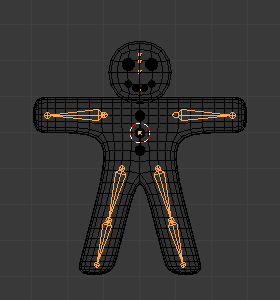
\includegraphics[width=0.4\textwidth]{resources/chapter-2-basic-armature.png}
    \caption{\textit{Skinned armature} sederhana \parencite{blender-armature-structure}}
    \label{fig:basic-armature}
\end{figure}

\begin{figure}[ht]
    \centering
    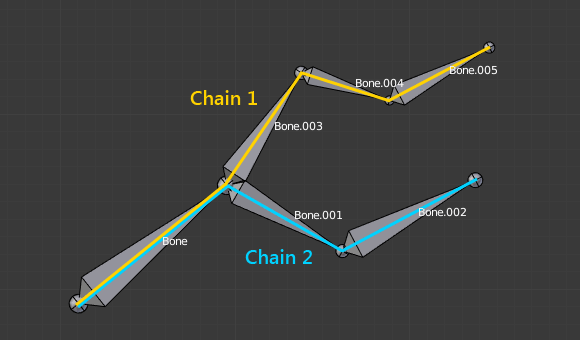
\includegraphics[width=0.6\textwidth]{resources/chapter-2-chain-of-bones.png}
    \caption{\textit{Chains of Bones} \parencite{blender-armature-structure}}
    \label{fig:chains-of-bones}
\end{figure}

\subsection{\textit{Bone}}

\textit{Bone} merupakan komponen dari \textit{armature}
\parencite{blender-bones-introduction}. Struktur sebuah \textit{bone} dapat
dilihat pada Gambar \ref{fig:bone-structure}. Sebuah \textit{bone} terdiri atas
3 subkomponen adalah sebagai berikut:
\parencite{blender-bones-structure,blender-glossary}:

\begin{enumerate}

    \item Sendi awal (\textit{root}/\textit{head})

    Sendi awal memiliki koordinat pada sumbu X, Y, dan Z di ruang lokal
    (\textit{local space}) objek \textit{armature}. Sendi awal merupakan titik
    acuan untuk rotasi \textit{bone} pada sumbu X dan Z pada (\textit{local
    space}). Rotasi ini disebut juga sebagai \textit{roll angle}.

    \item Sendi akhir (\textit{tip}/\textit{tail})

    Sendi akhir memiliki koordinat pada sumbu X, Y, dan Z relatif terhadap sendi
    awal.

    \item Badan (\textit{body})

    Badan oktahedral dari \textit{bone} terbentuk untuk menghubungkan sendi awal
    dan sendi akhir. Bagian sudut oktahedral yang lebih besar berhubungan
    dengan sendi awal. Sebaliknya, bagian sudut oktahedral yang lebih kecil
    berhubungan dengan sendi akhir. Badan \textit{bone} menentukan arah sumbu Y
    lokal dan rotasi \textit{bone} objek ketika diposekan.

\end{enumerate}

\begin{figure}[ht]
    \centering
    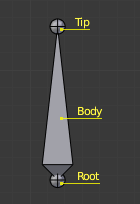
\includegraphics[width=0.3\textwidth]{resources/chapter-2-bone-structure.png}
    \caption{Struktur \textit{bone} \parencite{blender-bones-structure}}
    \label{fig:bone-structure}
\end{figure}

% \section{RoadRunner}
% RoadRunner merupakan sebuah \textit{interactive editor} yang digunakan untuk
% membuat konten desain 3D untuk simulasi dan pengujian sistem kendaraan otonom.
% Pengguna dapat membuat desain jalanan dengan mengedit lingkungan dan menambahkan
% rambu lalu lintas, sinyal lalu lintas, persimpangan, dan batas kendaraan. Selain
% itu, RoadRunner dapat digunakan untuk membuat desain kota \parencite{roadrunner}.

\section{Penelitian Terkait}

Subbab ini membahas beberapa penelitian terkait dengan Tugas Akhir ini.
Penelitian-penelitian berikut menjadi rujukan dalam penelitian dan pengembangan
Tugas Akhir ini.

\subsection{Pengembangan Sistem Otonomi dengan Menggunakan Kecerdasan Artificial untuk Trem}
\label{subsec:rispro-trilaksono}

Penelitian oleh \cite{rispro-trilaksono} merupakan penelitian mengenai inovasi
bidang otomotif yang mengembangkan sistem otonomi untuk trem menggunakan
kecerdasan buatan. Penelitian tersebut memiliki tiga tahap, yaitu pengembangan
\textit{tram driving assistance}, pengembangan trem otonom, dan pengujian trem
otonom di \textit{mixed traffic} serta persiapan komersialisasi.

Berikut Indikator Kinerja Riset (IKR) atau luaran penelitian tersebut
\parencite{rispro-trilaksono}:

\begin{enumerate}

    \item Pengembangan algoritma persepsi untuk mengenali objek dan
    \textit{tracking} di lingkungan trem pada cuaca normal dan implementasi
    dalam bentuk \textit{software}.

    % Algoritma persepsi yang dikembangkan berupa \textit{panoptic segmentation},
    % \textit{camera object detection}, \textit{LIDAR object detection},
    % \textit{camera-LIDAR fusion object detection}, dan \textit{camera-radar
    % fusion object detection}

    \item Pengembangan algoritma perencanaan jalur untuk \textit{decision
    making} kendali kecepatan trem dan implementasi dalam bentuk
    \textit{software}.

    % Algoritma persepsi yang dikembangkan berupa \textit{railway estimator},
    % \textit{trajectory prediction}, dan \textit{safety assessment}

    \item Pengambilan \textit{dataset} lingkungan trem

    \textit{Dataset} yang diambil bentuk gambar citra kamera biasa, gambar citra
    LIDAR, dan data lainnya kemudian diolah dengan penambahan anotasi
    seperlunya.

    \item Pengembangan \textit{Driving Assistance System} untuk trem berupa:
    \textit{object detection \& collision-avoidance assist}, \textit{speed limit
    assist}, dan \textit{face recognition \& driver attention warning}.

    \item Pengujian, analisis, dan desain ulang algoritma yang dikembangkan pada
    \textit{Software-in-the-Loop Simulation} (SILS) dan
    \textit{Hardware-in-the-Loop Simulation} (HILS).

    Menguji dan menganalisis \textit{platform} simulasi, yaitu simulator CARLA
    versi 0.9.12, uji coba beragam sensor, dan uji coba beberapa algoritma yang
    sudah dikembangkan. Melakukan konversi kode program/algoritma yang telah
    dikembangkan ke bahasa pemrograman C++ untuk dimasukkan ke NVIDIA DRIVE AGX
    Pegasus (selanjutnya akan disebut sebagai Pegasus) dan membuat
    \textit{web-service} untuk menghubungkan server simulasi dengan NVIDIA drive
    AGX Pegasus. Pegasus merupakan \textit{hardware} untuk memroses
    algoritma \textit{Adaptive Cruise Control} (ACC), \textit{Emergency Braking
    System} (EBS), dan \textit{Collision Avoidance} (\textit{decision making}).
    Dari pengujian dan analisis tersebut, dibutuhkan penyempurnaan algoritma
    persepsi berbasis sensor, perbaikan arsitekstur (HILS), dan integrasi objek
    lokal pada skenario simulasi.

    \item Pengembangan dan manufaktur \textit{platform} trem, sistem
    \textit{drive-by-wire} pada trem, dan integrasi sensor.

    \item Publikasi ilmiah.
    \item Draf kekayaan intelektual.
    \item \textit{Self-assessment} Tingkat Kesiapan Teknologi (TKT).
    \item Penyusunan poster ilmiah populer atas pelaksanaan dan hasil riset.

\end{enumerate}

\subsection{\textit{KIT Bus: A Shuttle Model for CARLA Simulator}}

Penelitian \textit{KIT Bus: A Shuttle Model for CARLA Simulator} ini merupakan
penelitian membuat model \textit{shuttle bus} untuk CARLA yang dilakukan oleh
\cite{related-work-xiang}. Proses pembuatan model tersebut dilakukan dalam tiga
tahap, yaitu sebagai berikut \parencite{related-work-xiang}:

\begin{enumerate}

    \item Membuat model 3D dari bus menggunakan aplikasi 3ds Max.

    Model bus dibuat sesuai dengan referensi dan dimensi asli. Model bus yang
    dibuat secara detil dan berpermukaan mulus sehingga realistis. Model bus
    terdiri atas 6 bagian, yaitu bagian badan, bagian roda-roda, bagian
    interior, bagian detil, bagian kaca, dan bagian plat kendaraan.

    \item Melakukan pengeditan model 3D bus dalam CARLAUE4.

    Model bus yang telah dibuat kemudian diimpor ke dalam CARLAUE4.
    Masing-masing bagian badan bus dan keempat roda bus dipasangkan sebuah
    \textit{collision box} yang berbentuk dan berukuran sama. Agar model bus
    dapat menyimulasikan animasi bus yang sebenarnya, \textit{Blueprint} animasi
    harus dibuat berbagai macam bagian bus yang bergerak. Dilakukan juga
    penambahan material atau tekstur dan fungsionalitas lainnya yang dibutuhkan
    seperti, lampu dan tekstur-tekstur yang ada pada permukaan bus. Hal tersebut
    dilakukan sehingga model bus dapat menyerupai model bus yang sebenarnya.
    Model bus yang telah selesai diedit dimasukkan ke dalam \textit{vehicle
    factory} agar dapat bisa dimunculkan (\textit{spawn}).

    \item Memverifikasi kontrol manual dan otonom dari model 3D bus yang telah
    dibangun dalam CARLA.

    Model bus yang telah dibuat kemudian diuji untuk memverifikasi apakah model
    bus tersebut dapat dioperasikan secara manual dan otonom. Model bus dites
    untuk berjalan maju, mengerem untuk melambat, mengemudi ke kiri dan ke
    kanan, dan memindahkan gigi kopling.

\end{enumerate}

\subsection{\textit{The Autonomous Siemens Tram}}

Penelitian \textit{The Autonomous Siemens Tram} membahas trem otonom Siemens
yang telah didemonstrasikan di Potsdam, Jerman pada tahun 2018. Sistem trem
otonom tersebut dibangun di atas trem Siemens Combino dan menggunakan
sensor-sensor multi-modal untuk mengidentifikasi lokasi kendaraan serta
mendeteksi dan merespon lampu lalu lintas dan objek lain. Trem otonom memiliki
beberapa komputer yang memiliki \textit{Graphics Processing Unit} (GPU) yang
memadai untuk memroses data dari sensor LIDAR, sensor radar, kamera pendeteksi
objek, dan kamera pendekteksi sinyal. Trem otonom tersebut dapat beroperasi
dengan lancar namun memiliki kendala ketika melakukan lokalisasi trem hanya
dengan Global Navigation Satellite System (GNSS). Penelitian masih dilakukan
untuk mengatasi kendala tersebut, misalnya dengan melakukan lokalisasi dengan
persepsi atau visual \parencite{at-palmer}.

% \blankpage
\chapter{Deskripsi Solusi}
\label{chapter-3}

Bab ini membahas deskripsi umum permasalahan \textit{capstone}, analisis masalah
simulasi yang sudah ada, analisis terhadap objek dan lingkungan yang akan
diimplementasi, analisis solusi yang akan diterapkan untuk mengatasi masalah.

\section{Deskripsi Umum Permasalahan \textit{Capstone}}

Proyek trem otonom menggunakan simulasi untuk mempercepat dan mempermudah
pengujian dan validasi pengembangan model/algoritma \textit{decision making},
persepsi, \textit{localization}, dan \textit{mapping} trem otonom. Tim
\textit{capstone} Tugas Akhir ini merupakan bagian dari tim simulasi yang
bertugas untuk mengembangkan simulasi yang sudah ada. Kemajuan
pengembangan simulasi atau pengembangan SILS dan HILS adalah sebagai berikut:

\begin{enumerate}

	\item Eksplorasi kakas CARLA sebagai simulator.

	CARLA versi 0.9.12 diinstal. Model angkot dan becak telah diimpor
	sebagai objek statis (bukan kendaraan). Kendaraan model \textit{FireTruck}
	digunakan sebagai \textit{ego vehicle} menggantikan trem untuk sementara
	waktu karena model trem belum diintegrasi sebagai kendaraan.

	\item \textit{Web service} telah diimplementasi sebagai jalur komunikasi
	antara simulator CARLA dan Pegasus pada HILS.

	Komunikasi menggunakan \textit{web service} lambat karena jumlah transaksi
	per detik kecil dan simulasi juga lambat. Eksplorasi CARLA ROS Bridge
	dilakukan namun belum selesai.

	\item Menguji sensor virtual, mencoba menjalankan algoritma \textit{decision
	making} dan persepsi.

	Sensor virtual diuji apakah layak untuk digunakan sebagai pengganti sensor
	asli. Algoritma \textit{decision making} dan persepsi diuji juga pada HILS.

	\item Membuat rancangan skenario simulasi.

	Rancangan daftar skenario simulasi untuk menguji berbagai skenario dengan
	variabel cuaca, waktu, kecepatan trem, dan lalu lintas yang berbeda.

\end{enumerate}

Dari kemajuan proyek dari tahun sebelumnya dibutuhkan  penyempurnaan algoritma
persepsi berbasis sensor, perbaikan arsitektur HILS atau komunikasi yang
memadai, dan integrasi objek lokal pada skenario simulasi. Tim \textit{capstone}
yang beranggotakan 3 orang bertanggung jawab untuk:

\begin{enumerate}

	\item Mengembangkan mekanisme komunikasi antarperangkat dalam arsitektur
	HILS yang lebih lancar dan lebih cepat.
	\item Membuat implementasi skenario pengujian simulasi.
	\item Mengintegrasikan dan/atau mengimplementasikan objek lokal ke skenario
	simulasi.

\end{enumerate}

Tugas Akhir ini bertujuan untuk mengimplementasikan objek trem, objek lokal
lingkungan Indonesia di simulasi menggunakan CARLA agar lingkungan simulasi
menyerupai lingkungan aslinya sehingga mendukung pengembangan pengujian dan
validasi \textit{decision making} dan persepsi dengan menggunakan simulasi.

\section{Analisis Masalah Simulasi dan Aset Simulasi}

Simulasi trem otonom untuk saat ini telah diinisiasi namun baru sebatas
eksplorasi simulator CARLA dengan menambahkan kendaraan angkot dan becak sebagai
objek statis (bukan kendaraan) dan mengetes data dari sensor di \textit{ego
vehicle} dalam simulasi. Aset model 3D sudah dibangun namun belum
diimplementasikan ke dalam simulasi. Aset model 3D tersebut adalah: trem,
angkot, becak, sepeda onthel, sepeda motor, beberapa rambu lalu lintas, dan
gerobak. Gambar \ref{fig:3d-model-assets} menunjukkan aset model 3D yang telah
dibuat.

\begin{figure}[!tb]
% \begin{figure}[ht]
	\centering
	\subfloat[Trem]{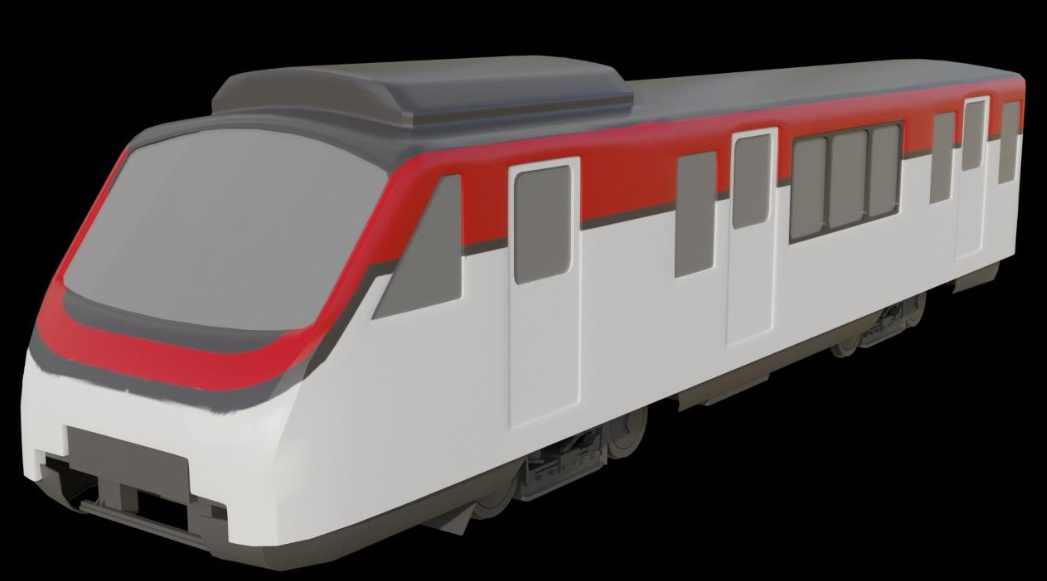
\includegraphics[width=0.4\textwidth]{resources/chapter-3-tram.png}}
	\hfill
	\subfloat[Angkot]{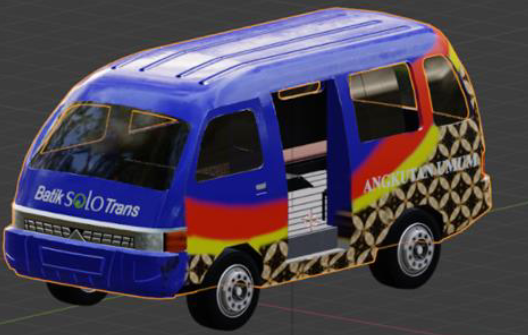
\includegraphics[width=0.4\textwidth]{resources/chapter-3-angkot.png}}
	\hfill
	\subfloat[Becak]{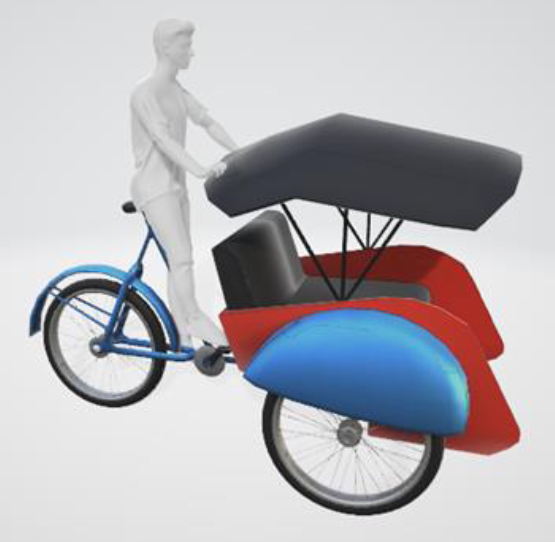
\includegraphics[width=0.3\textwidth]{resources/chapter-3-becak.png}}
	\hfill
	\subfloat[Sepeda onthel]{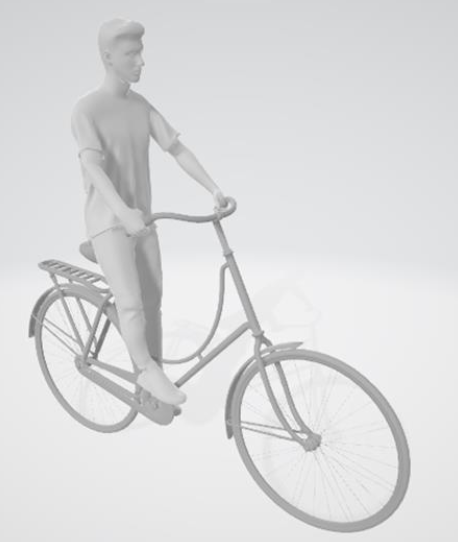
\includegraphics[width=0.3\textwidth]{resources/chapter-3-sepeda-onthel.png}}
	\hfill
	\subfloat[Sepeda motor]{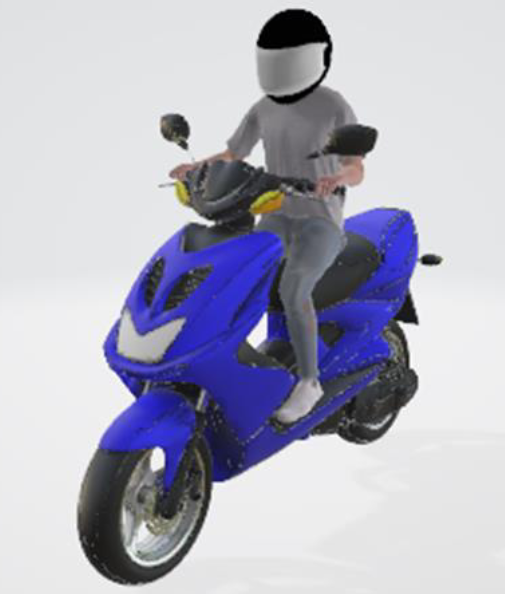
\includegraphics[width=0.3\textwidth]{resources/chapter-3-sepeda-motor.png}}
	\hfill
	\subfloat[Rambu-rambu lalu lintas]{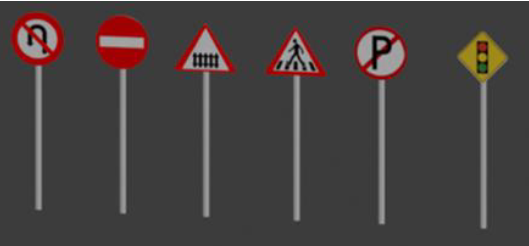
\includegraphics[width=0.4\textwidth]{resources/chapter-3-rambu.png}}
	\hfill
	\subfloat[Gerobak]{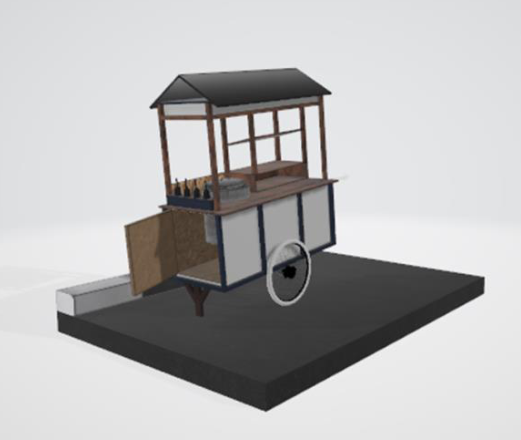
\includegraphics[width=0.4\textwidth]{resources/chapter-3-gerobak.png}}
	\caption{Aset model 3D \parencite{rispro-trilaksono}}
	\label{fig:3d-model-assets}
\end{figure}

Selain aset angkot dan becak yang diimpor sebagai objek statis, aset simulasi
untuk saat ini baru berupa aset bawaan dari CARLA. Aset bawaan CARLA seperti
peta kota, kendaraan, bangunan, rambu lalu lintas, dan lain-lain merupakan aset
yang mencerminkan kota-kota di Amerika Serikat pada umumnya. Implementasi objek
dan lingkungan Indonesia dibutuhkan agar simulasi serupa dengan kehidupan nyata
di Indonesia sehingga ketika pengujian strategi kemudi trem otonom memiliki
tingkat akurasi dan presisi yang tinggi. Simulasi yang sesuai dengan keadaan
aslinya sangat berpengaruh terhadap sistem trem otonom. Diperlukan penambahan
aset model 3D lain yang juga perlu diimplementasikan pada simulasi. Aset
tersebut adalah stasiun trem, rel trem, dan rambu yang lengkap.

Modul simulasi ini merupakan bagian dari pengembangan sistem otonom dengan
menggunakan kecerdasan buatan untuk trem. Modul ini bertujuan untuk memenuhi
kebutuhan pengujian virtual strategi kemudi trem otonom dengan simulasi.
Simulasi ini bertujuan untuk melakukan validasi strategi kemudi kecerdasan
buatan trem otonom yang telah dikembangkan. Validasi diperlukan agar kecerdasan
buatan yang dikembangkan dapat beroperasi dengan lancar di lingkungan Indonesia.
Oleh karena itu, dibutuhkan aset simulasi yang sesuai dengan keadaan Indonesia.

\section{Analisis Solusi}

Permasalahan yang telah dibahas dapat diselesaikan dengan mengedit aset yang
sudah ada dan menambahkan aset baru. Aset baru yang lain dapat dibuat
menggunakan aplikasi \textit{3D modelling}. Aset dibuat secara lengkap dan
detail agar perilaku aset sesuai dengan yang asli.

% the sentence below goes after the first sentence
% Aset seperti peta kota harus dibuat langsung menggunakan editor CARLAUE4 atau
% menggunakan RoadRunner kemudian diimpor ke dalam editor CARLAUE4 jika aset
% peta diperlukan.

Aset model 3D yang telah jadi selanjutnya diimpor ke dalam editor CARLAUE4.
Proses impor aset ini dilakukan dengan mengikuti panduan yang telah tersedia di
dokumentasi CARLA. Proses impor aset harus dilakukan dengan benar agar perilaku
aset baik dan stabil untuk simulasi. Terdapat aset khusus yang harus ditambahkan
ke dalam berkas 3D model kendaraan dan diatur ke model kendaraan. Aset khusus
tersebut merupakan aset \textit{armature} untuk \textit{rigging} roda kendaraan.
Setelah pengaturan aset dalam editor CARLAUE4 selesai, dilakukan verifikasi aset
dengan cara menjalankan simulasi dan mengamati cara kendaraan beroperasi.
Implementasi aset berupa kendaraan bus telah berhasil dilakukan pada penelitian
lain yang dibahas pada Subbab \ref{subsec:kitbus}. Proses implementasi kendaraan
bus dilakukan dengan membuat model 3D bus, mengimpor model 3D bus ke dalam
editor CARLAUE4, mengedit aset bus tersebut dalam editor CARLAUE4, dan
memverifikasi hasil impor aset bus tersebut.

% Implementasi objek dan lingkungan Indonesia yang akan dilakukan adalah dengan
% menambahkan/mengimpor aset, membuat aset baru, dan mengedit aset yang sudah ada.
% Implementasi yang menambahkan aset meliputi kendaraan, rambu lalu lintas, rel,
% dan stasiun. Kendaraan yang akan diimplementasikan adalah trem otonom, angkot,
% becak, motor, dan sepeda onthel.
% Trem akan dipasangkan berbagai sensor, seperti LIDAR, radar, kamera RGB untuk
% menangkap lingkungan sekitar.

% note: gerobak is not going to be implemented

Penambahan atau pengeditan aset CARLA membutuhkan simulator CARLA, CARLAUE4, dan
editor CARLAUE4 yang dibangun atau di-\textit{compile} sendiri bukan menggunakan
program, \textit{binary}, atau yang sudah \textit{packaged}. Dibutuhkan aplikasi
\textit{3D modelling} seperti Blender untuk membuat aset model 3D.
% Aplikasi RoadRunner akan digunakan untuk membuat aset peta.

\section{Rancangan Implementasi Objek dan Lingkungan Indonesia di Simulator CARLA}

Proses implementasi objek dan lingkungan di simulator CARLA dilakukan dengan
langkah-langkah sebagai berikut:

\begin{enumerate}

	\item Eksplorasi editor CARLAUE4 versi 0.9.12 dan versi 0.9.13.

	Eksplorasi dilakukan untuk memelajari cara menggunakan editor CARLAUE4 dan
	mengetahui fitur-fitur yang telah dikembangkan oleh tim pengembang CARLA.

	\item Membuat aset baru dengan Blender.

	Aset baru yang dibutuhkan dibuat mengikuti dokumentasi CARLA mengenai
	penambahan aset-aset yang bersangkutan. Aset baru yang butuh
	diimplementasikan adalah stasiun trem, rel trem, dan rambu lalu lintas.
	% Hal tersebut meliputi bentuk poligon, jumlah poligon, jumlah VEF, dan
	% lain-lain. (yang sesuai dengan petunjuk)

	\item Melakukan impor dan edit aset ke dalam editor CARLAUE4.

	Aset yang ingin dimasukkan ke lingkungan simulasi dan diedit harus dilakukan
	dengan aplikasi CARLAUE4.

	% aset carla berbentuk .uasset yang merupakan binary file

	% untuk import vehicles:
	% https://carla.readthedocs.io/en/0.9.13/tuto_A_add_vehicle/#bind-and-model-the-vehicle
	% ~~untuk buat peta:~~
	% ~~https://carla.readthedocs.io/en/0.9.13/tuto_M_generate_map/~~

	% links:
	% https://carla.readthedocs.io/en/0.9.13/tuto_A_add_props/
	% https://carla.readthedocs.io/en/0.9.13/tuto_A_material_customization/

	\item Melakukan penambahan dan validasi aset yang telah diimpor.

	Aset yang telah diimpor dimasukkan ke dalam lingkungan simulasi
	(\textit{world}). Validasi aset dapat dilakukan dengan menjalankan simulator
	dan mengamati aset dalam simulasi. Validasi ini dilakukan untuk memastikan
	aset yang diimpor dan ditambahkan sudah sesuai dengan yang diinginkan dan
	stabil dalam simulasi.

	\item Melakukan ekspor hasil implementasi agar dapat didistribusikan.

	Aset yang ingin digunakan oleh pengguna lain dapat diekspor dalam bentuk
	versi \textit{packaged} sehingga \textit{portable} dan ringan ketika
	dijalankan. Hal ini dapat dilakukan dengan menjalankan perintah di terminal.

\end{enumerate}

\chapter{Implementasi dan Evaluasi}

\section{Hasil Eksplorasi CARLA}

Setelah membaca dokumentasi CARLA, menginstal CARLAUE4, dan mengeksplorasi
CARLAUE4 diketahui terdapat beberapa fitur sebagai berikut:

\begin{enumerate}
	\item Penambahan kendaraan baru beroda empat dan dua.
	\item Penambahan \textit{spline} untuk menambahkan rel.
	\item Penambahan objek statis lainnya.
\end{enumerate}

% TODO: tambah hasil eksplorasi lainnya
% TODO: ? BP, factory, spline

% TODO: ? cara import aset yang lain (yang khusus, yang detail di bawah aja)
% TODO: ? jelasin how to? but where

\section{Implementasi Trem dan Angkot}

\subsection{Pembuatan Aset Model 3D untuk Ekspor FBX}

Implementasi trem dan angkot mengikuti langkah-langkah pada
\textcite{blender-add-a-new-vehicle}. Pembuatan \textit{mesh} model 3D perlu
sesuai dengan persyaratan dari CARLA, yaitu jumlah tris (segitiga satuan yang
membentuk permukaan) adalah 50.000-100.000 dan melakukan pemisahan
material/tekstur sesuai dengan bagian kendaraan agar tampilan sesuai saat
disimulasikan.

Setelah model 3D dibuat, aset \textit{vehicle skeleton} atau \textit{armature}
dari \cite{blender-add-a-new-vehicle} perlu ditambahkan, diatur posisi
\textit{bone} dari \textit{armature}, dan dihubungkan ke \textit{mesh} model 3D.
Gambar \ref{fig:vehicle-skeleton} menunjukkan aset yang harus ditambahkan pada
kendaraan. Setelah \textit{armature} ditambahkan, masing-masing \textit{head}
dari \textit{bone} roda perlu diposisikan di tengah ban (lihat Gambar
\ref{fig:armature-placement}). Aset \textit{armature} hanya boleh ditranslasi
dan tidak boleh dirotasi ataupun diatur skalanya karena akan merusak proses
impor nantinya.

\begin{figure}[!h]
	\centering
	\subfloat[\textit{Armature}]{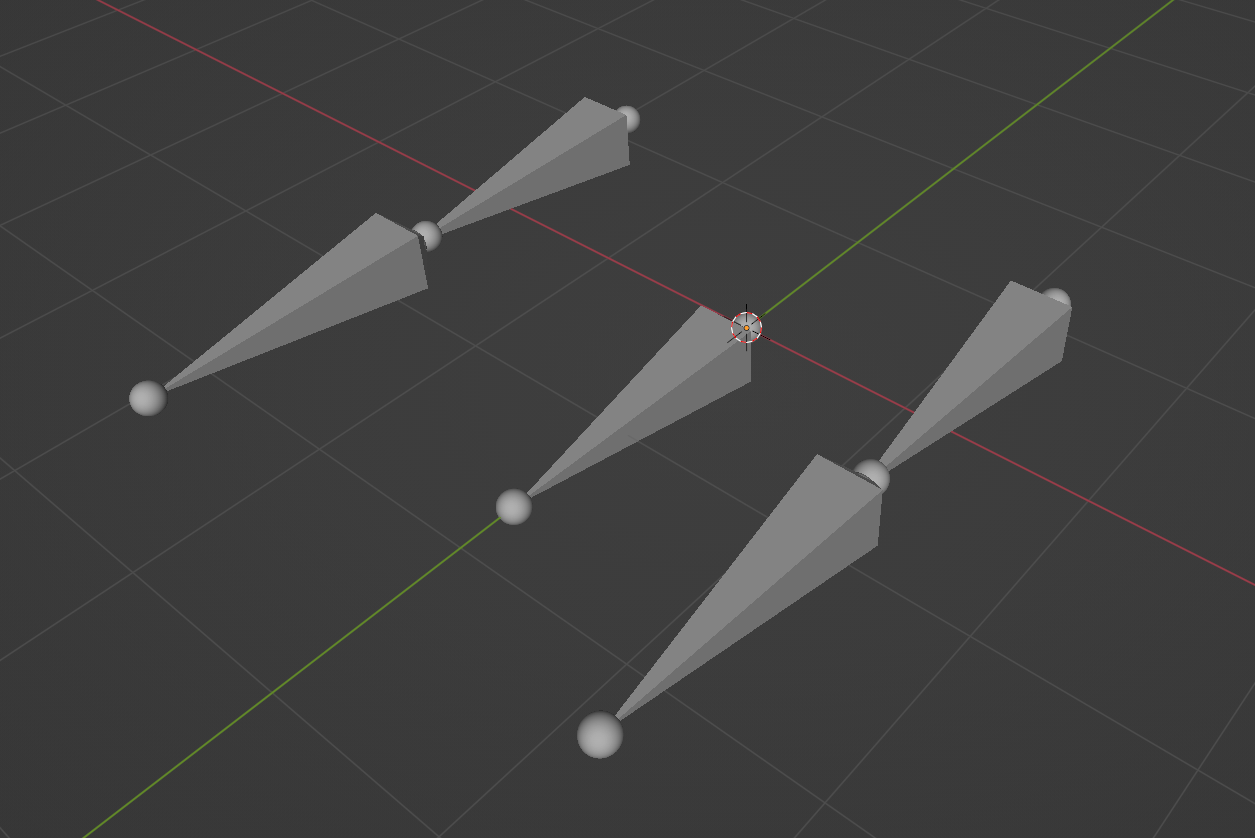
\includegraphics[width=0.45\textwidth]{resources/chapter-4/vehicle-skeleton.png}}
	\hfill
	\subfloat[Hierarki \textit{Vehicle skeleton}]{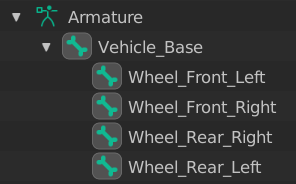
\includegraphics[width=0.45\textwidth]{resources/chapter-4/vehicle-skeleton-hierarchy.png}}
	\caption{\textit{Vehicle skeleton} kendaraan roda empat}
    \label{fig:vehicle-skeleton}
\end{figure}

\begin{figure}[!h]
	\centering
	\subfloat[Tampak samping roda depan kiri angkot]{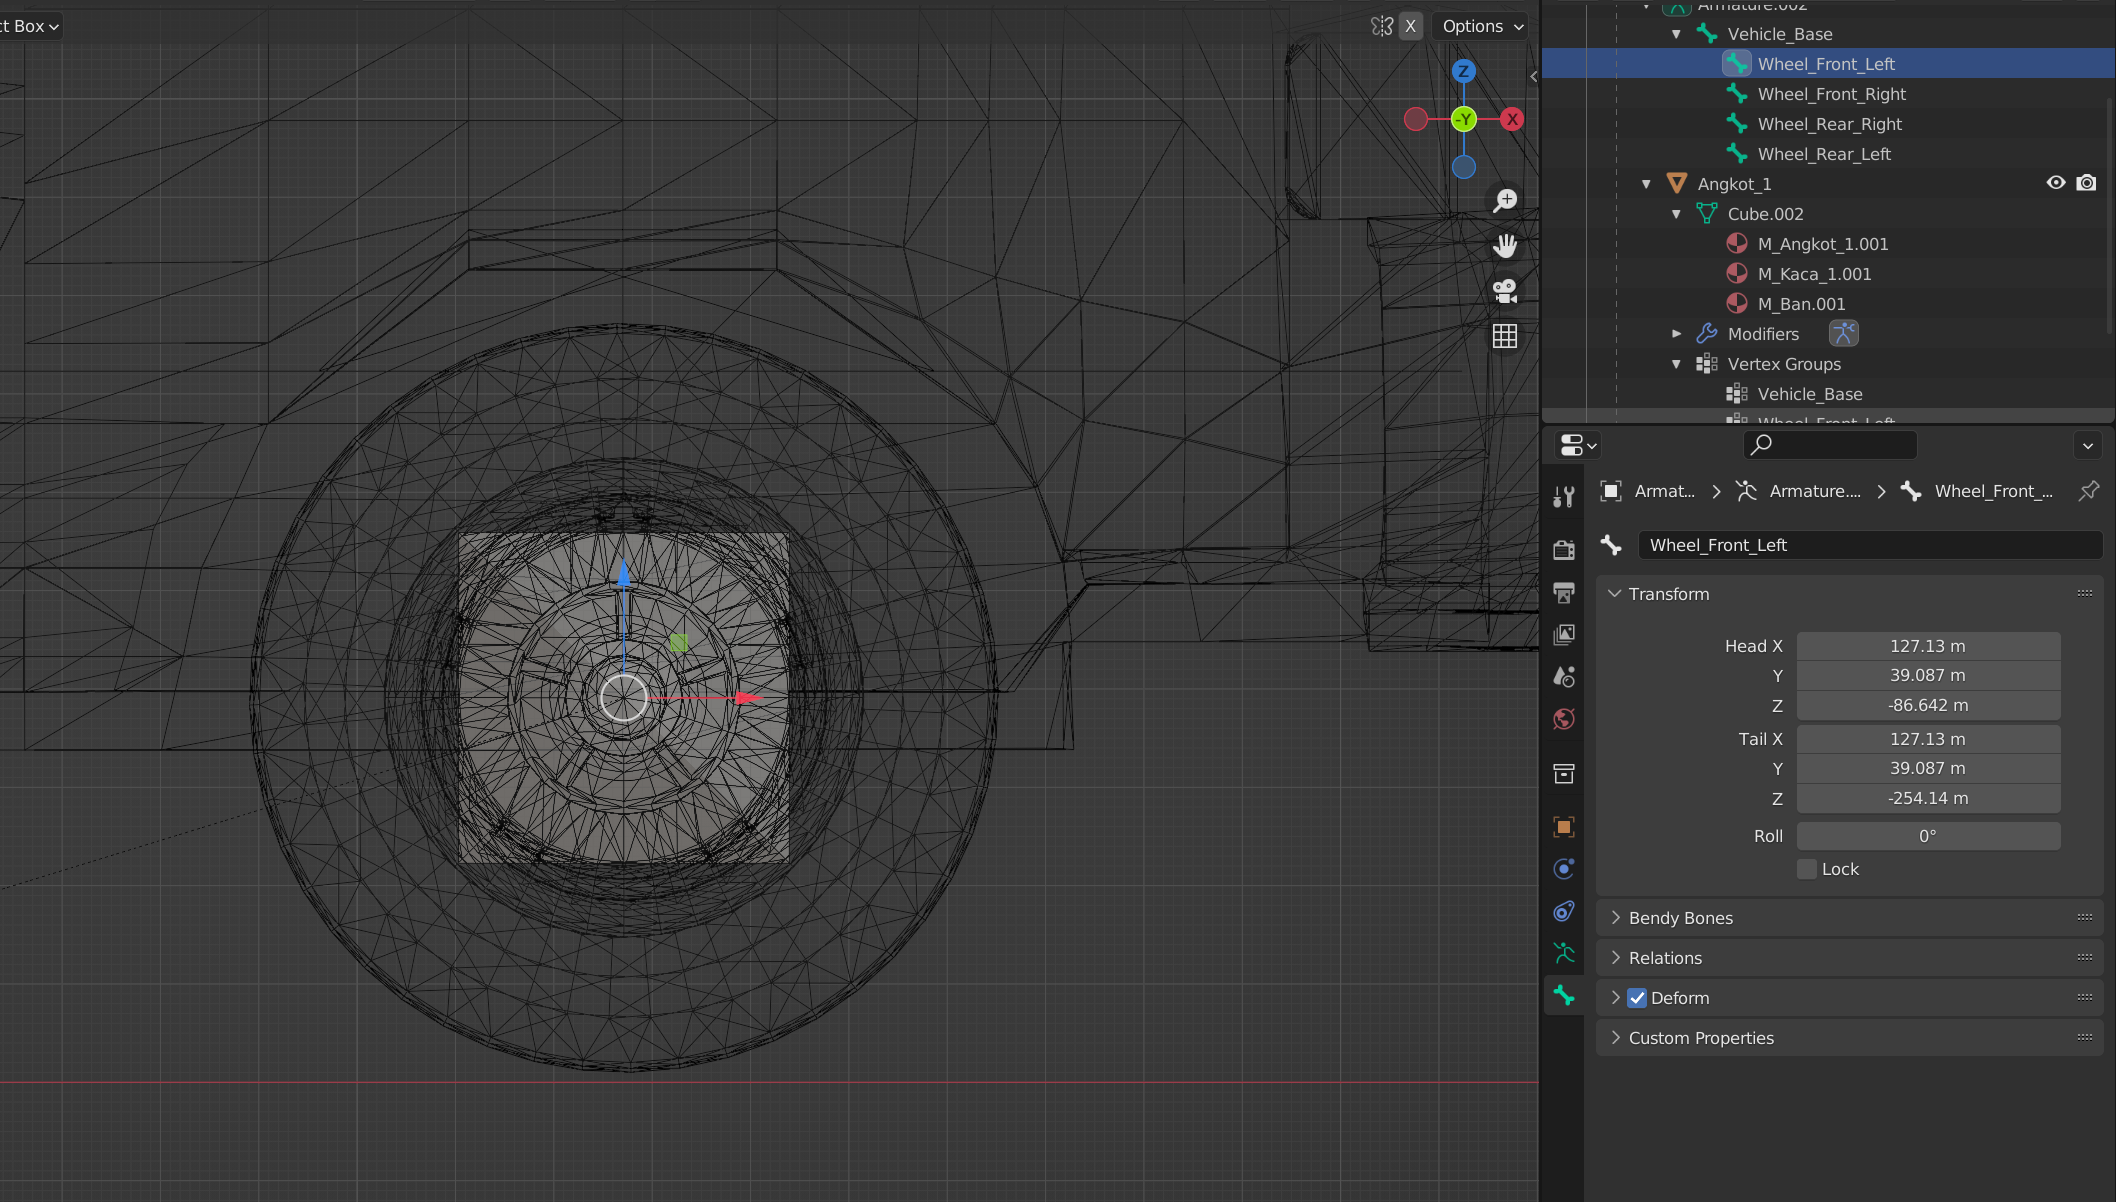
\includegraphics[width=0.45\textwidth]{resources/chapter-4/bone-placement-2.png}}
	\hfill
	\subfloat[Tampak depan roda depan kiri angkot \textit{Vehicle skeleton}]{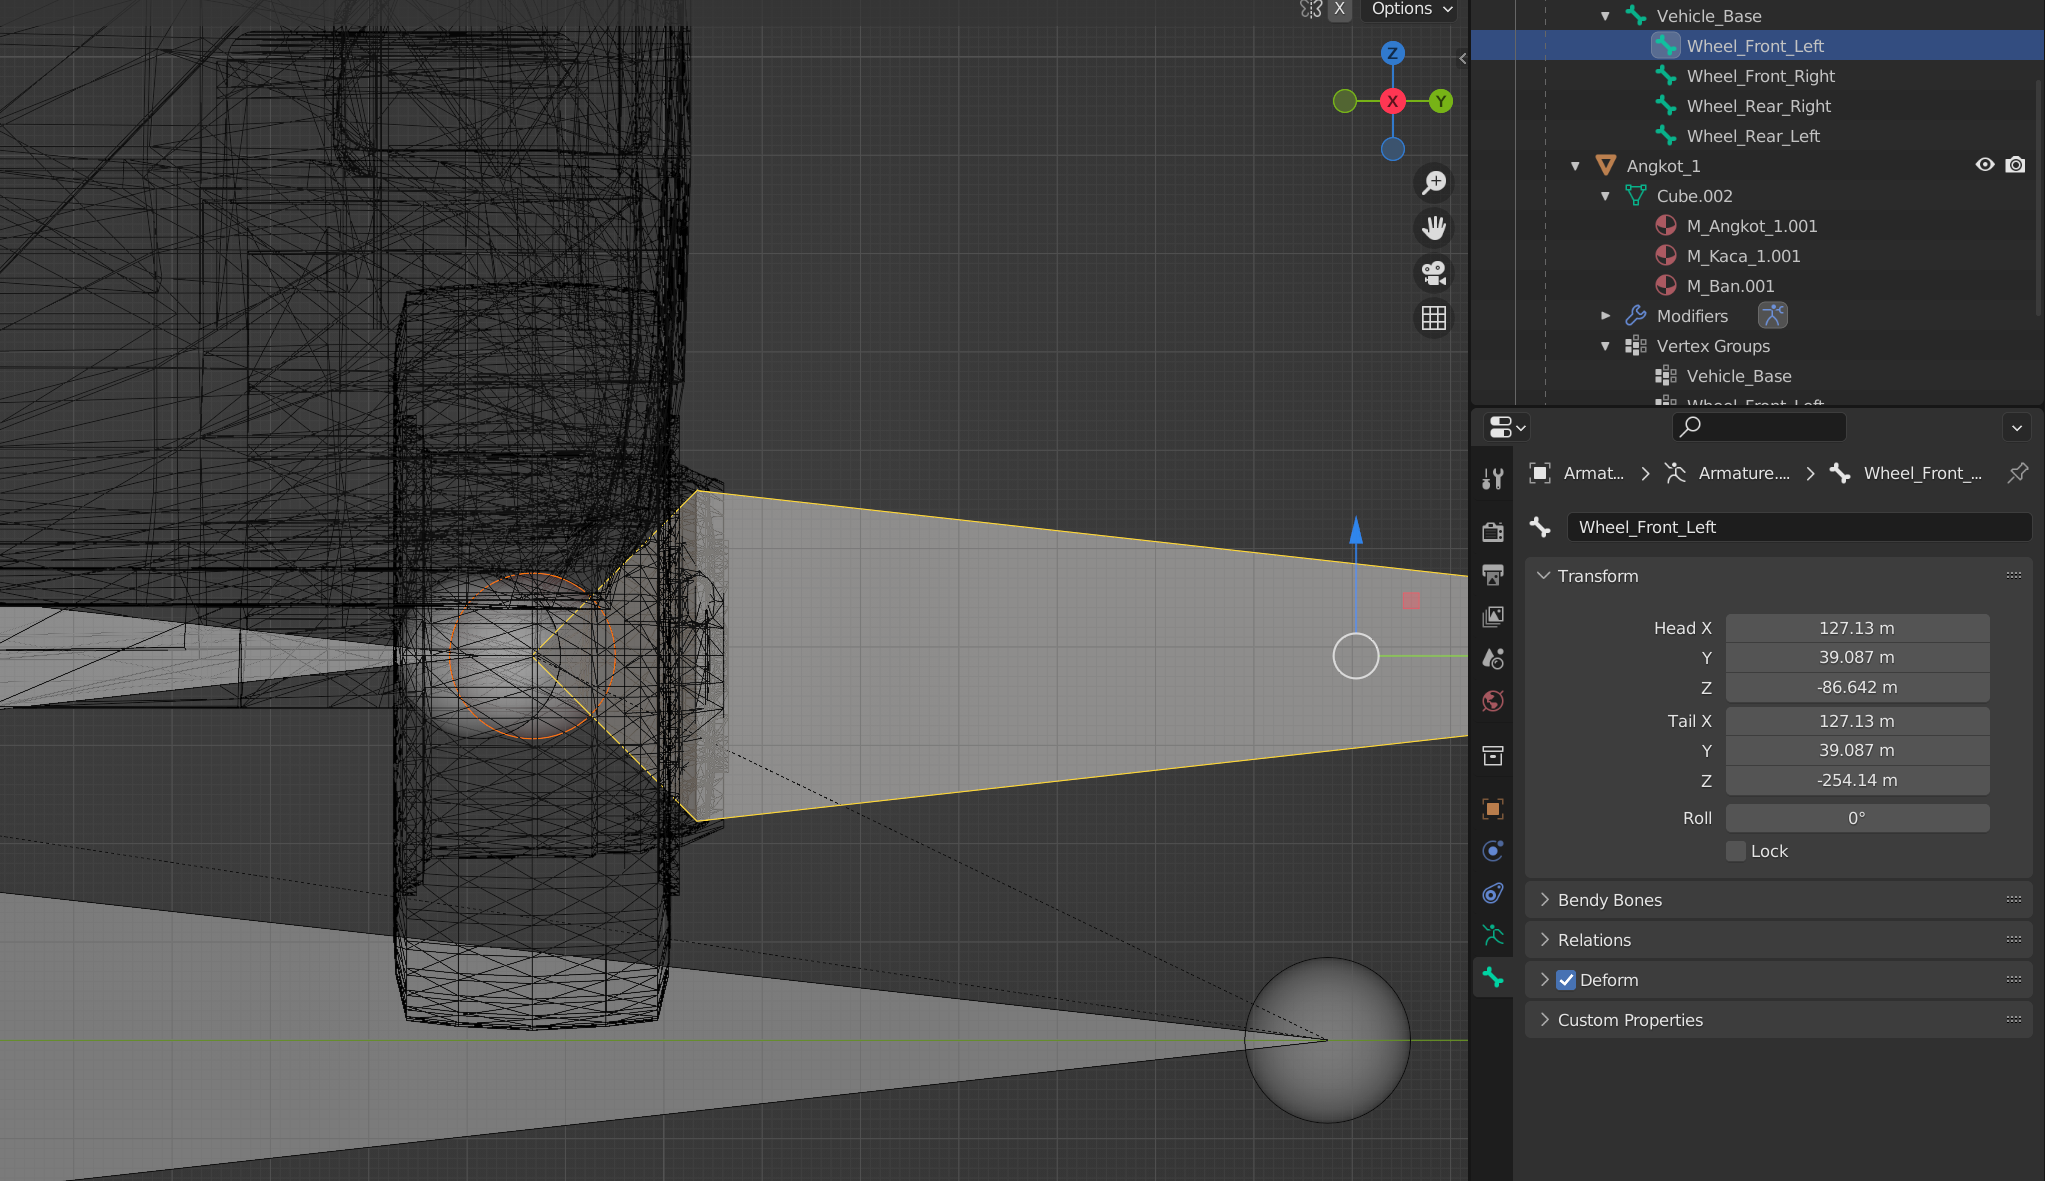
\includegraphics[width=0.45\textwidth]{resources/chapter-4/bone-placement-1.png}}
	\hfill
	\subfloat[Trem dengan \textit{armature}]{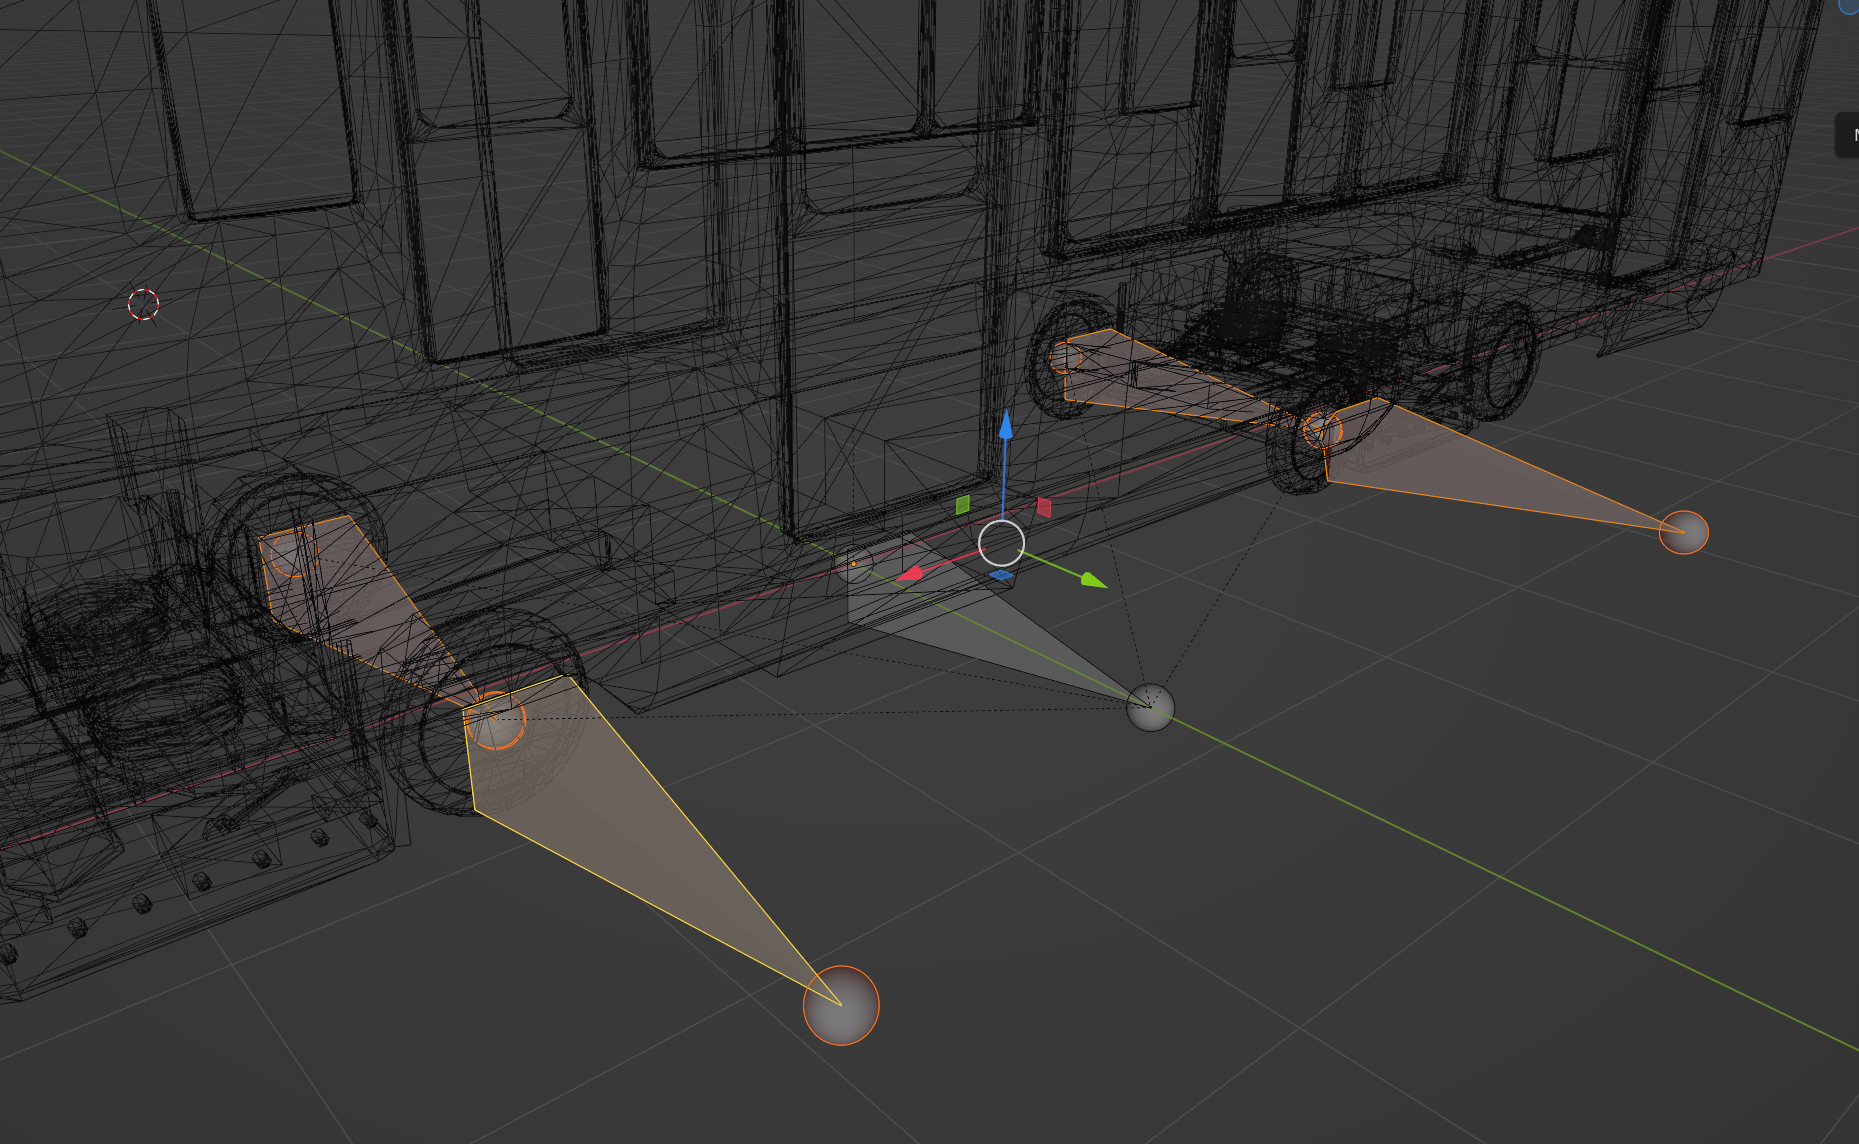
\includegraphics[width=0.45\textwidth]{resources/chapter-4/tram-wheels-bone.png}}
	\caption{Penempatan \textit{armature}}
    \label{fig:armature-placement}
\end{figure}

% TODO: cara skinning di blender
% TODO: cara membuat vertices groups

Setelah semua posisi \textit{bone} sesuai, dilakukan \textit{skinning}
\textit{armature} dengan \textit{mesh} kendaraan. Lima \textit{vertices groups}
dibuat untuk menghubungkan grup-grup dengan \textit{bone} yang sesuai. Kelima
\textit{vertices groups} dibuat dengan nama yang sesuai dengan nama
\textit{bone} yang akan dihubungkan. Gambar \ref{fig:vertices-groups}
menunjukkan \textit{vertices groups} yang sudah dibuat dan ditambahkan kumpulan
titiknya. Cara membuat \textit{vertices groups} adalah dengan memilih mode edit
(pada mesh kendaraan) dan menambahkan \textit{vertices groups} pada \textit{tab}
dengan nama \textit{Object Data Properties}. Setelah itu, \textit{vertices
groups} tersebut perlu diisi dengan titik-titik yang sesuai.

\begin{figure}[!h]
	\centering
    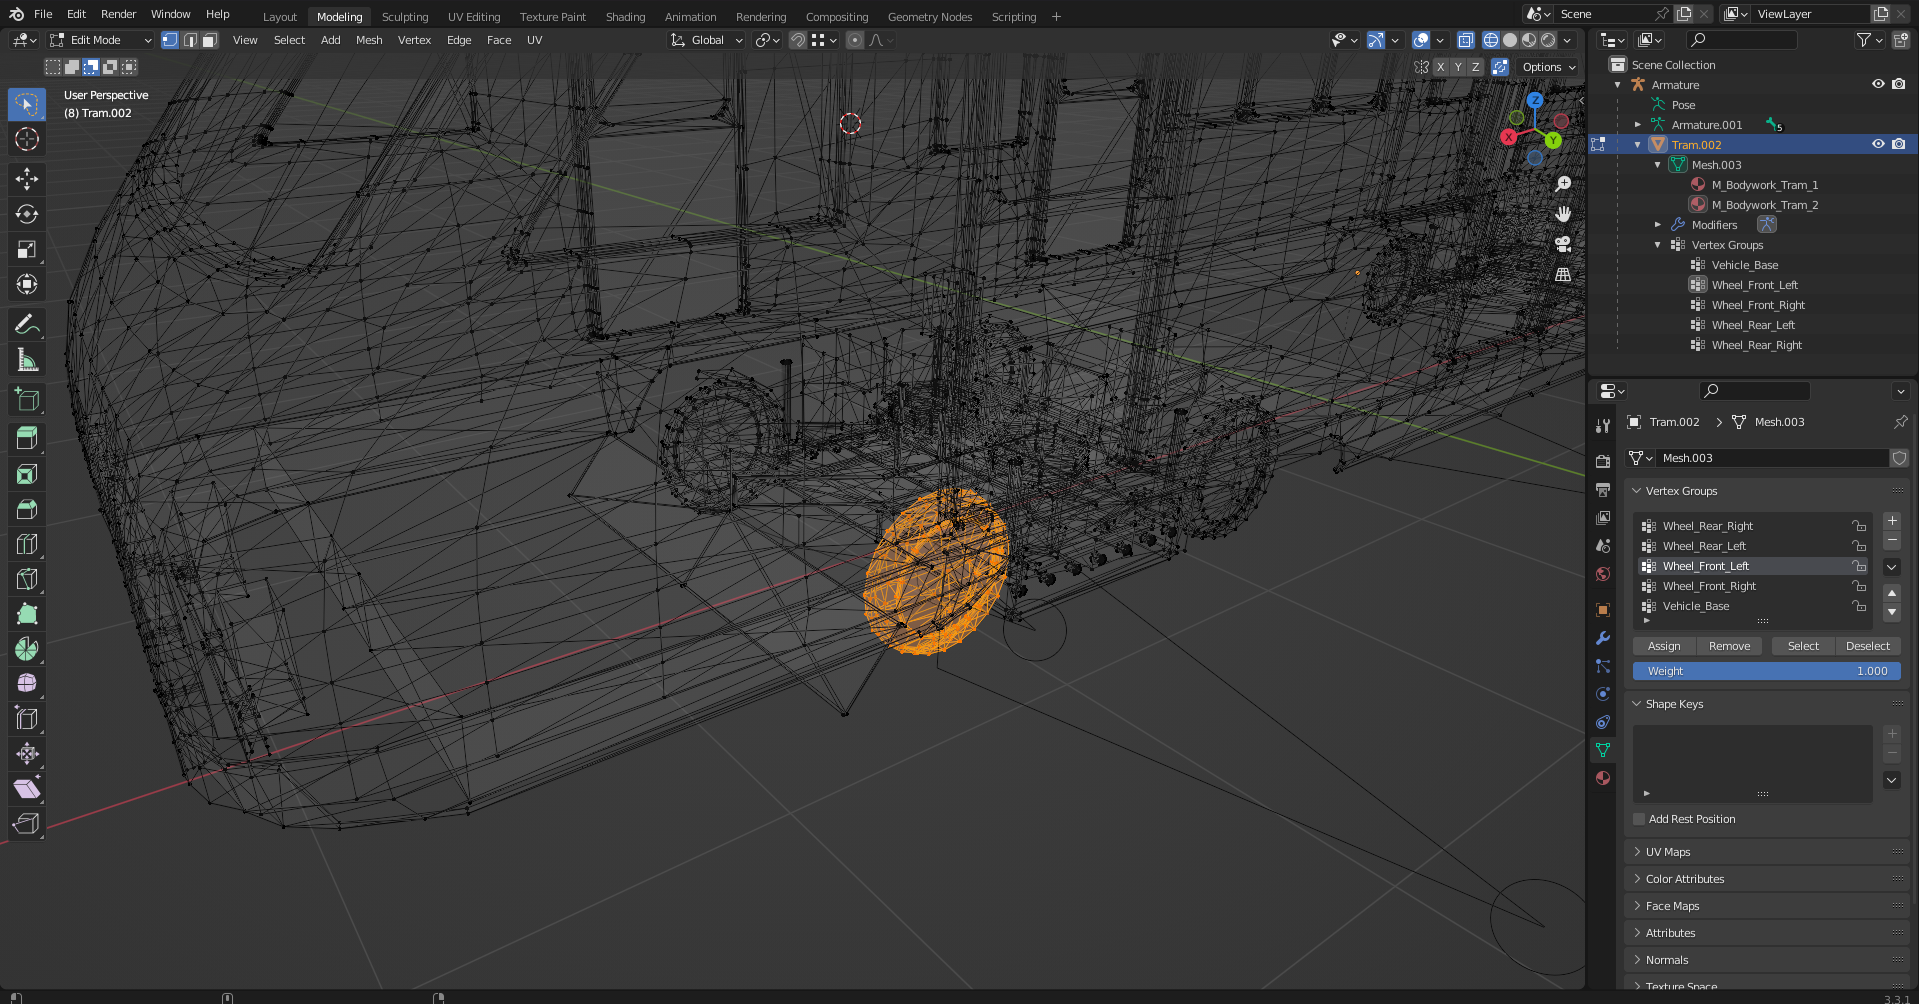
\includegraphics[width=1\textwidth]{resources/chapter-4/vertices-groups.png}
    \caption{Membuat \textit{vertices groups}}
	\label{fig:vertices-groups}
\end{figure}

Gambar \ref{fig:skinning-process} menunjukkan cara \textit{skinning}. Cara
melakukan \textit{skinning} adalah dengan menyusun hierarki objek seperti pada
Gambar \ref{fig:skinning-process} kemudian memilih menu \textit{Object},
\textit{Parent}, dan \textit{Armature Deform With Automatic Weights}
yang terletak pada \textit{Viewport Header}.

\begin{figure}[!h]
	\centering
    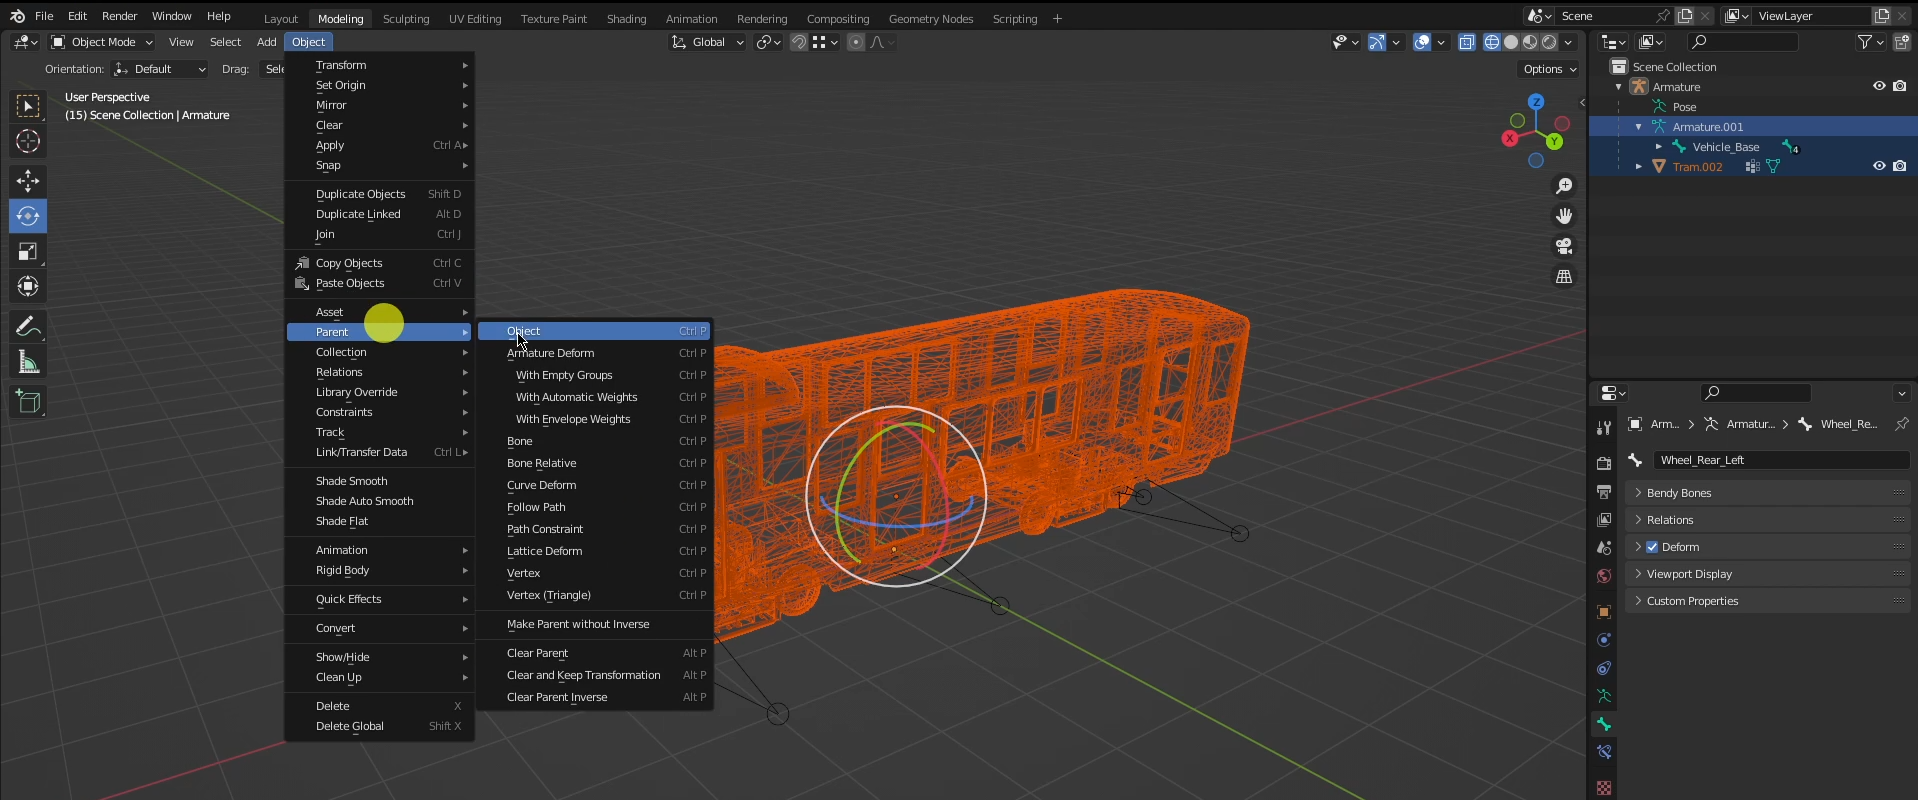
\includegraphics[width=1\textwidth]{resources/chapter-4/skining.png}
    \caption{\textit{Skinning}}
	\label{fig:skinning-process}
\end{figure}

Gambar \ref{fig:wheel-skinning} menunjukkan roda angkot bagian depan kiri yang
sudah dihubungkan dengan \textit{bone} yang sesuai. Pengujian ini dilakukan pada
\textit{pose mode}, memilih salah satu \textit{bone}, mengetik 'r', dan
menggerakan \textit{cursor}.

\begin{figure}[!h]
	\centering
	\subfloat[Roda posisi awal]{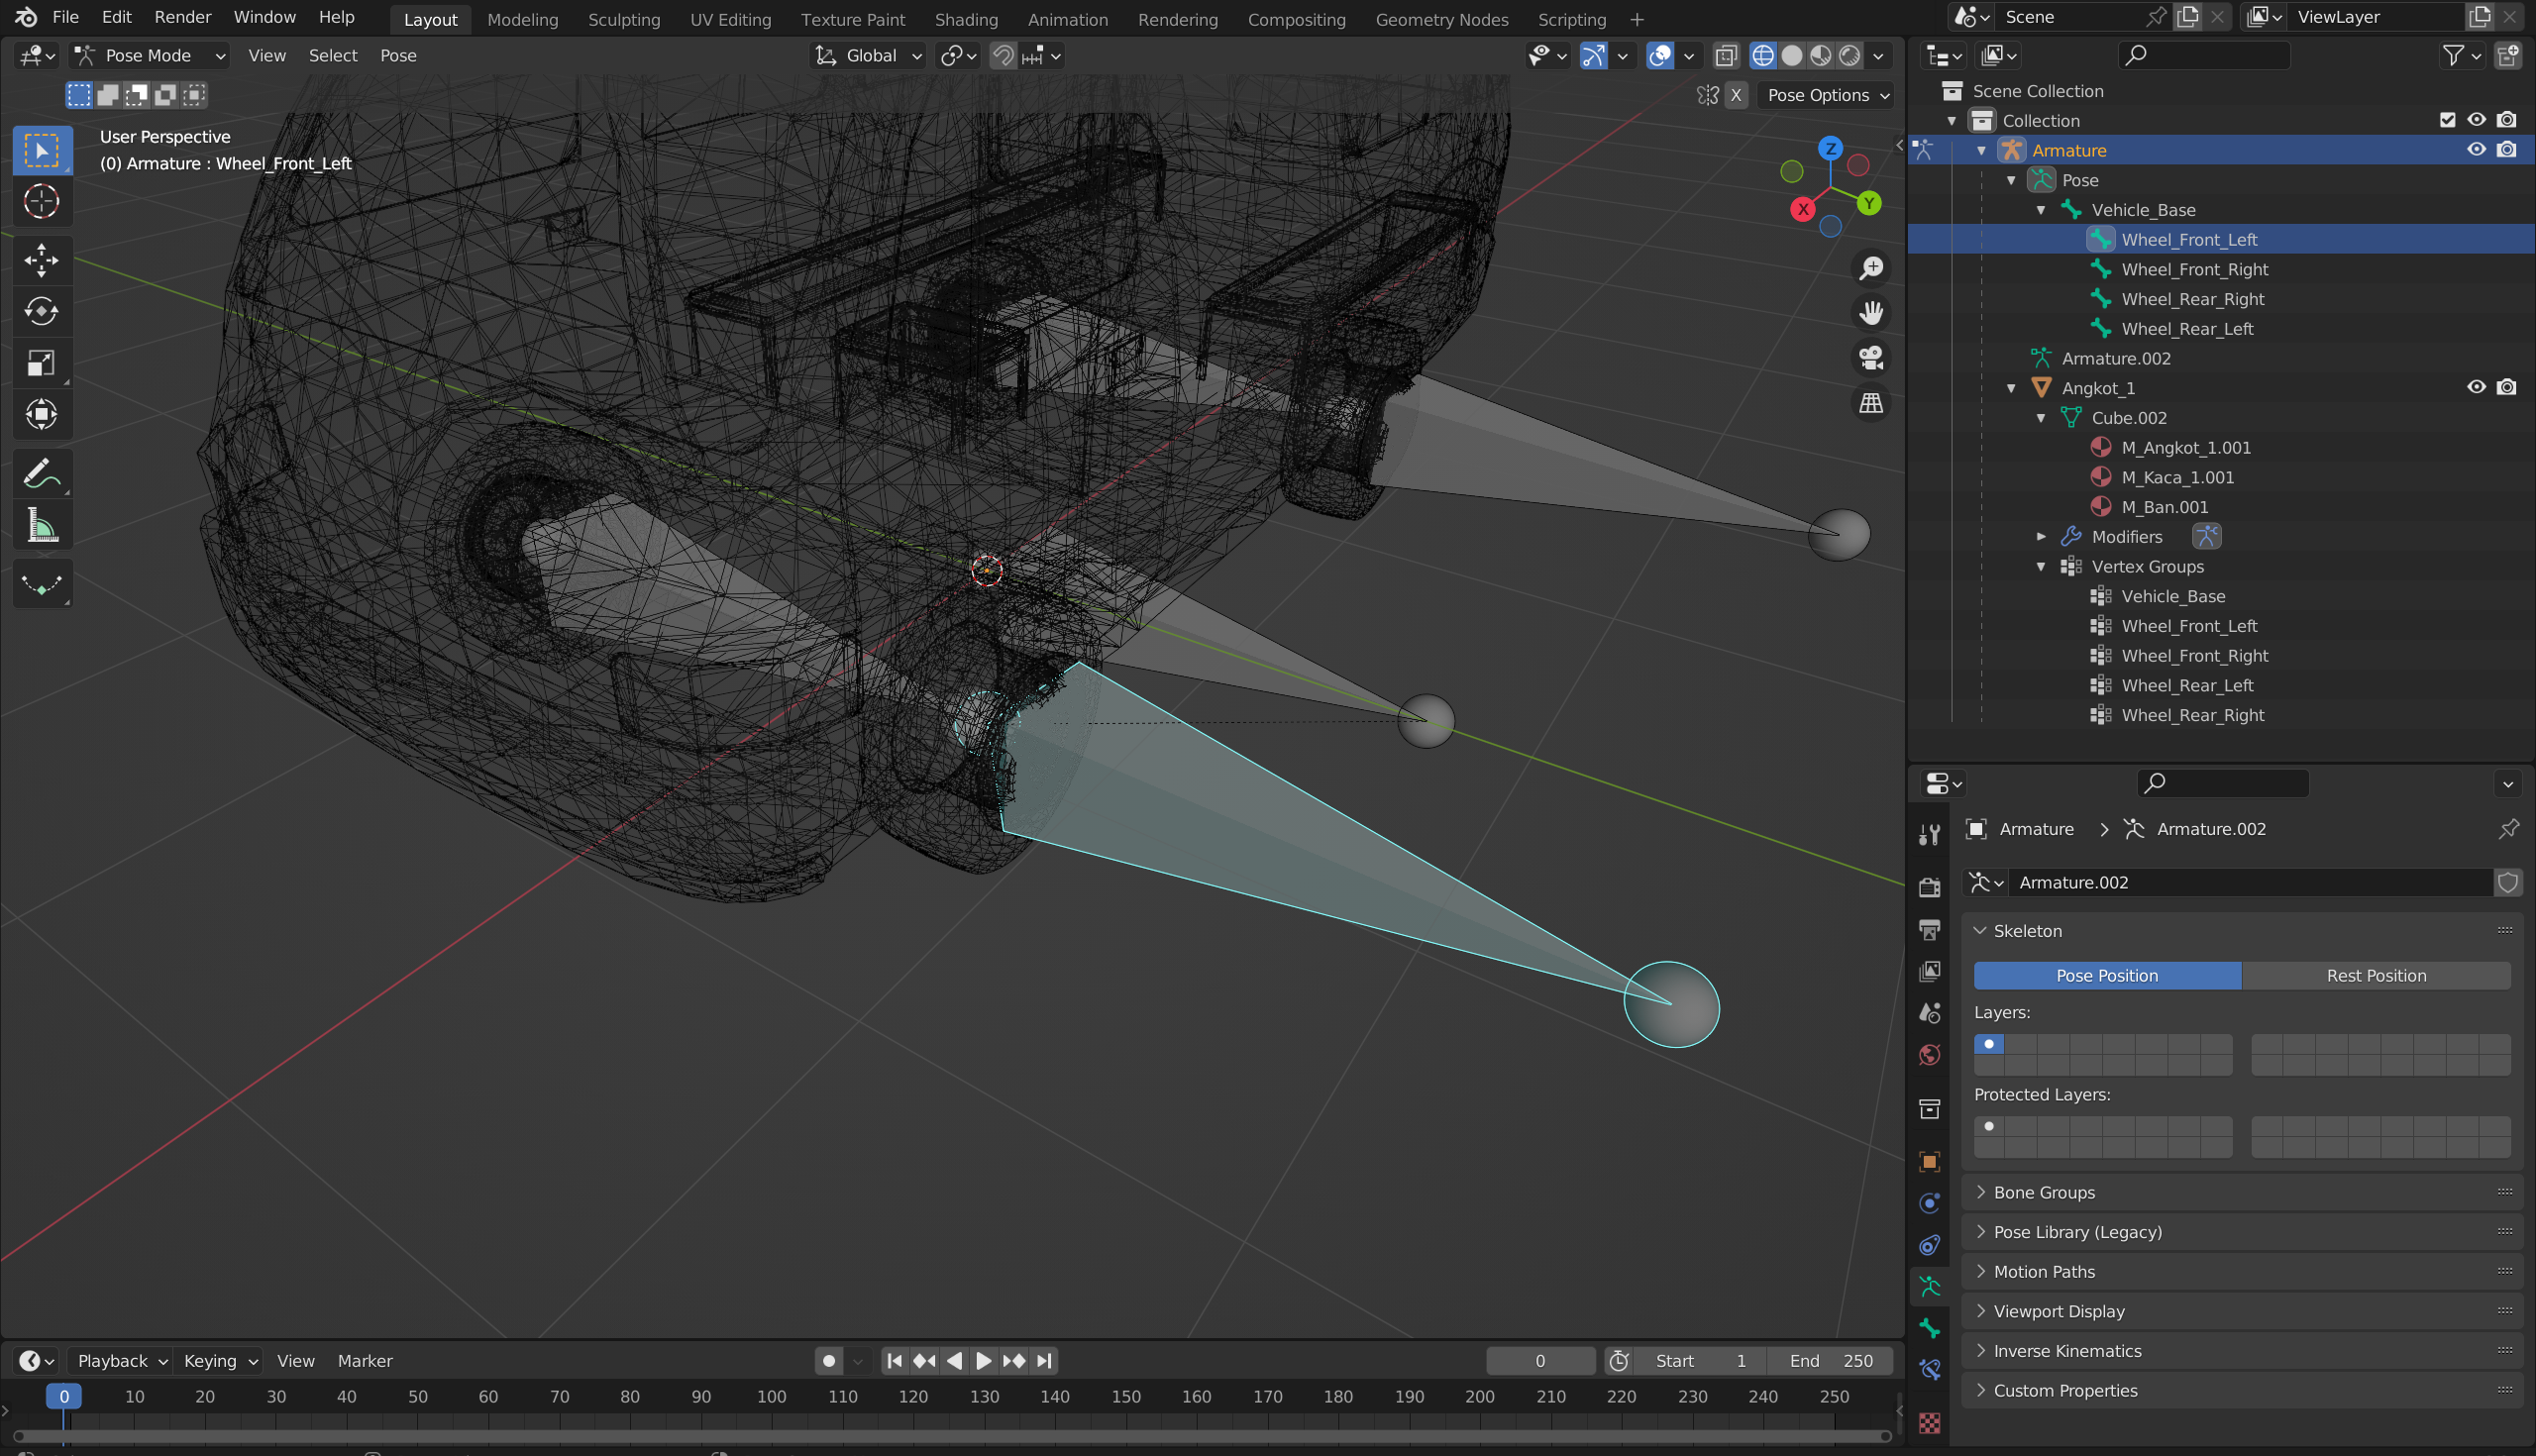
\includegraphics[width=0.47\textwidth]{resources/chapter-4/skinned-wheel-default.png}}
	\hfill
	\subfloat[Perubahan posisi roda]{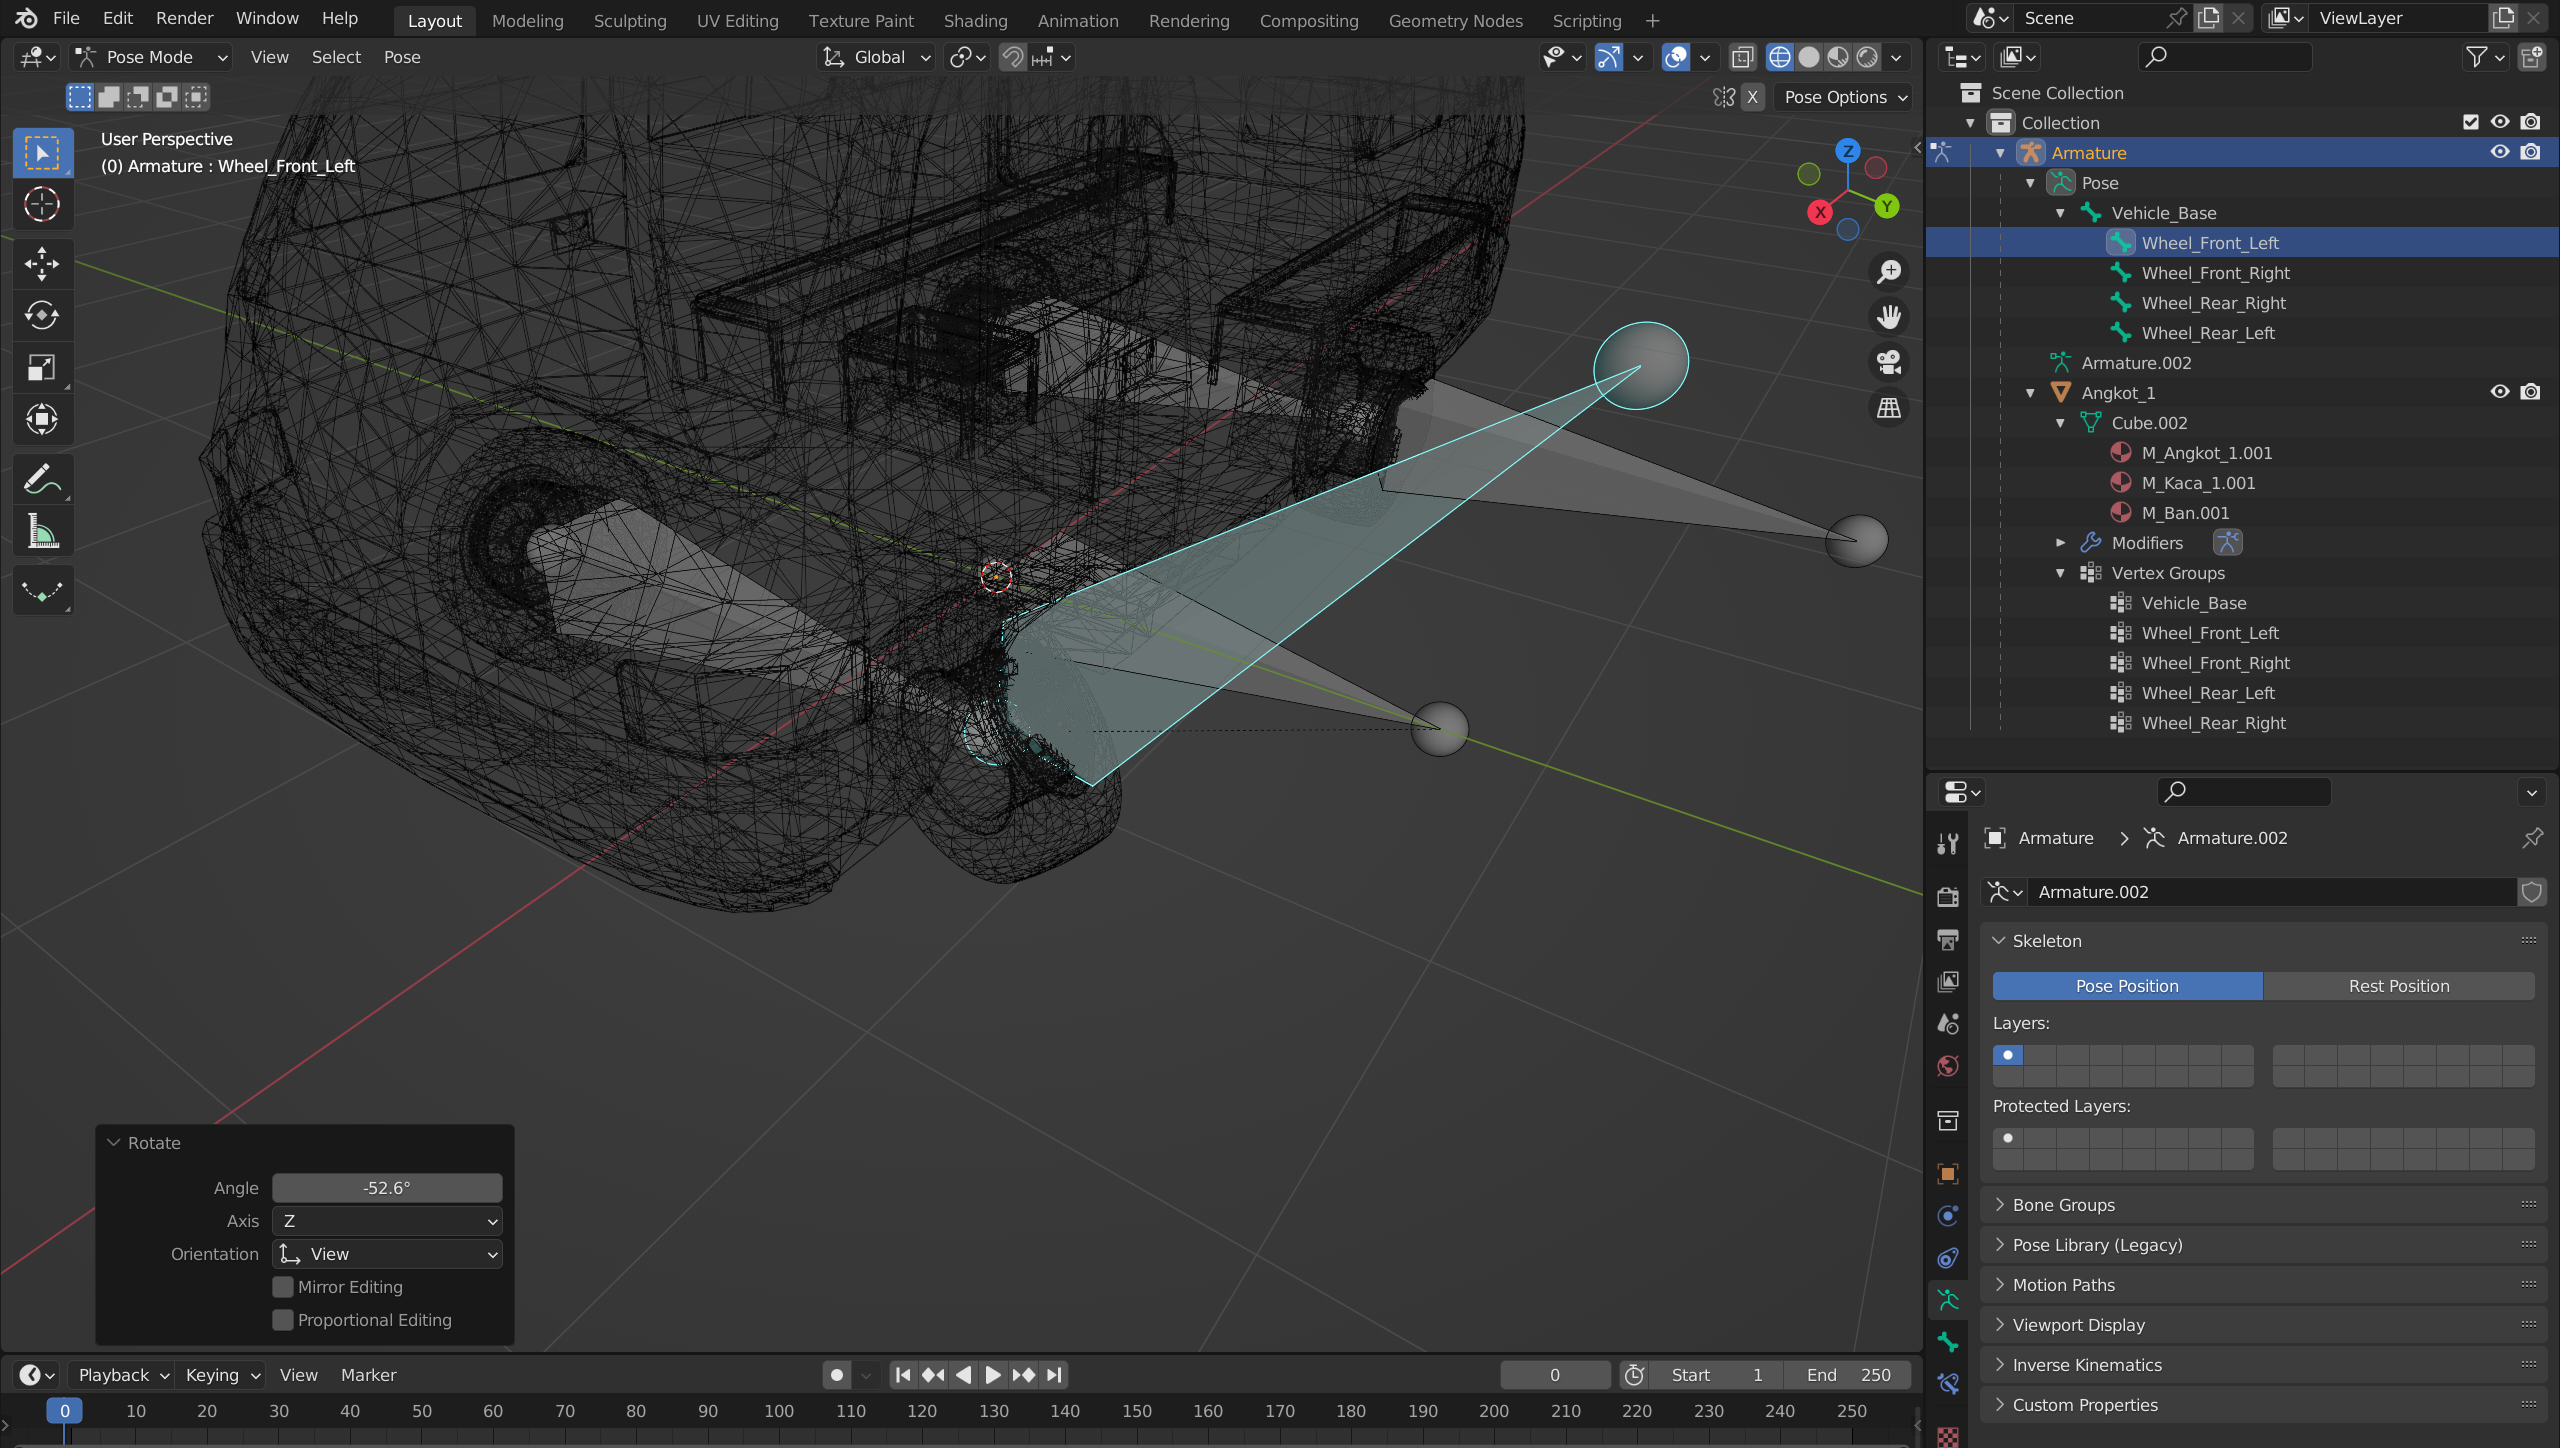
\includegraphics[width=0.47\textwidth]{resources/chapter-4/skinned-wheel-moved.png}}
	\caption{Hasil \textit{skinning} roda yang benar}
	\label{fig:wheel-skinning}
\end{figure}

Aset model 3D dapat diekspor ke dalam format FBX dengan cara memilih pilihan
pada Gambar \ref{fig:export-fbx}.

\begin{figure}[!h]
	\centering
	\subfloat[Opsi ekspor FBX]{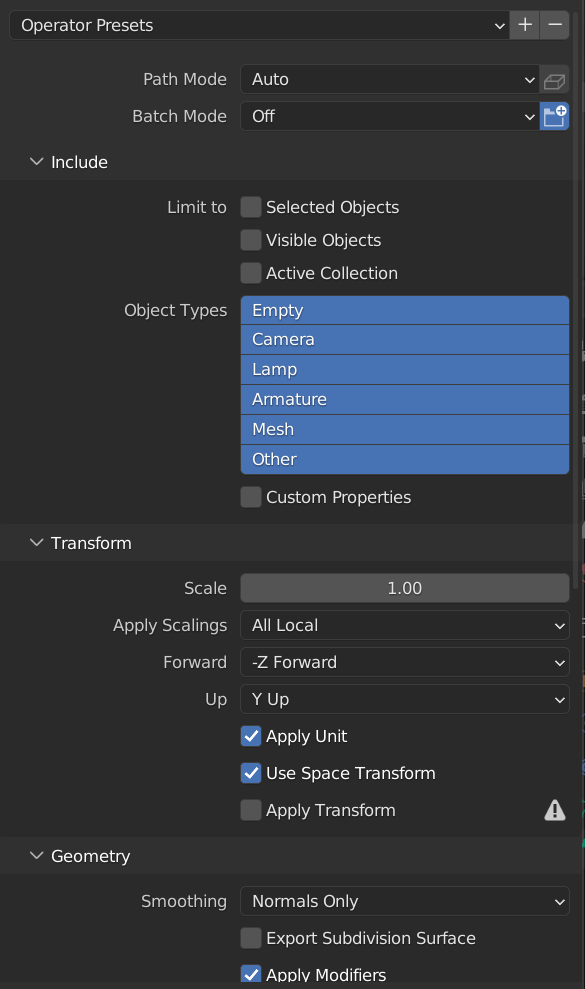
\includegraphics[width=0.47\textwidth]{resources/chapter-4/export-fbx-options-1.png}}
	\hfill
	\subfloat[Opsi ekspor FBX lanjutan]{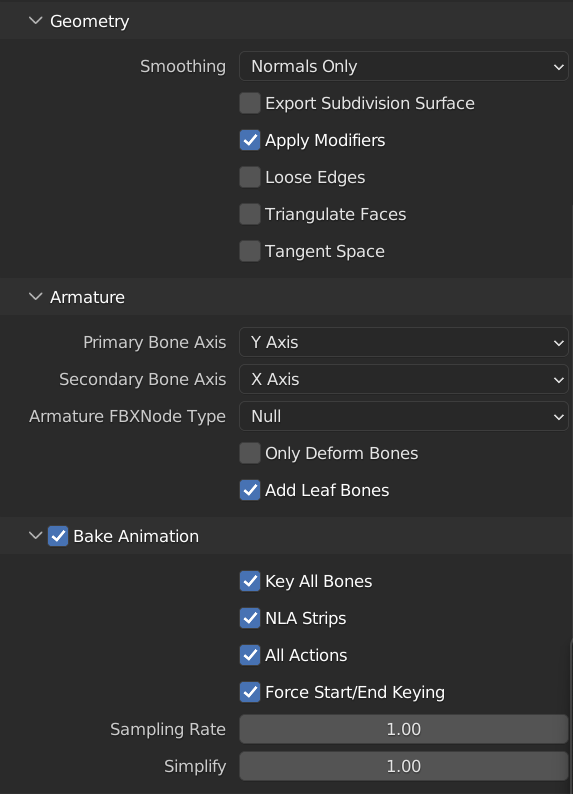
\includegraphics[width=0.47\textwidth]{resources/chapter-4/export-fbx-options-2.png}}
	\caption{Opsi ekspor FBX}
	\label{fig:export-fbx}
\end{figure}

\clearpage

\subsection{Impor Berkas FBX ke CARLAUE4}

Setelah aset model 3D selesai dibuat dan diekspor ke dalam format FBX, berkas
FBX tersebut diimpor ke dalam CARLAUE4. Berikut adalah langkah implementasi:

% TODO: buat jadi subsubsection?
\begin{enumerate}

    \item Buat \textit{folder} dengan nama \verb|<nama_kendaraan>| di direktori
    \verb|Content/Carla/Static/Vehicles/4Wheeled| di \textit{Content Browser}.
    \item Impor berkas FBX ke dalam \textit{folder} tersebut dengan klik kanan
    pada \textit{Content Browser}

    % many more + pics
    \dots

\end{enumerate}

\dots

% TODO: trouble shooting? hal2 yang harus diperhatikan

% new folder
% import + options
% buat animation blueprint
% make static mesh buat ganti ...
% set physical asset mesh

% navigate ke bp folder
% buat folder baru
% buat bp roda, bp kendaraan + configs

% add dto vehicle factory

% spawn vehicle (implemented but does it work?)

% \section{Sepeda Onthel, Sepeda Motor, dan Becak}
% \subsection{Pembuatan Aset Model 3D untuk Ekspor FBX}
% \subsubsection{Impor Berkas FBX ke CARLAUE4}

Gambar \ref{fig:tram-carla} menunjukkan hasil implementasi trem. Gambar
\ref{fig:angkot-carla} menunjukkan hasil implementasi trem  angkot.

\begin{figure}[!h]
    \centering
    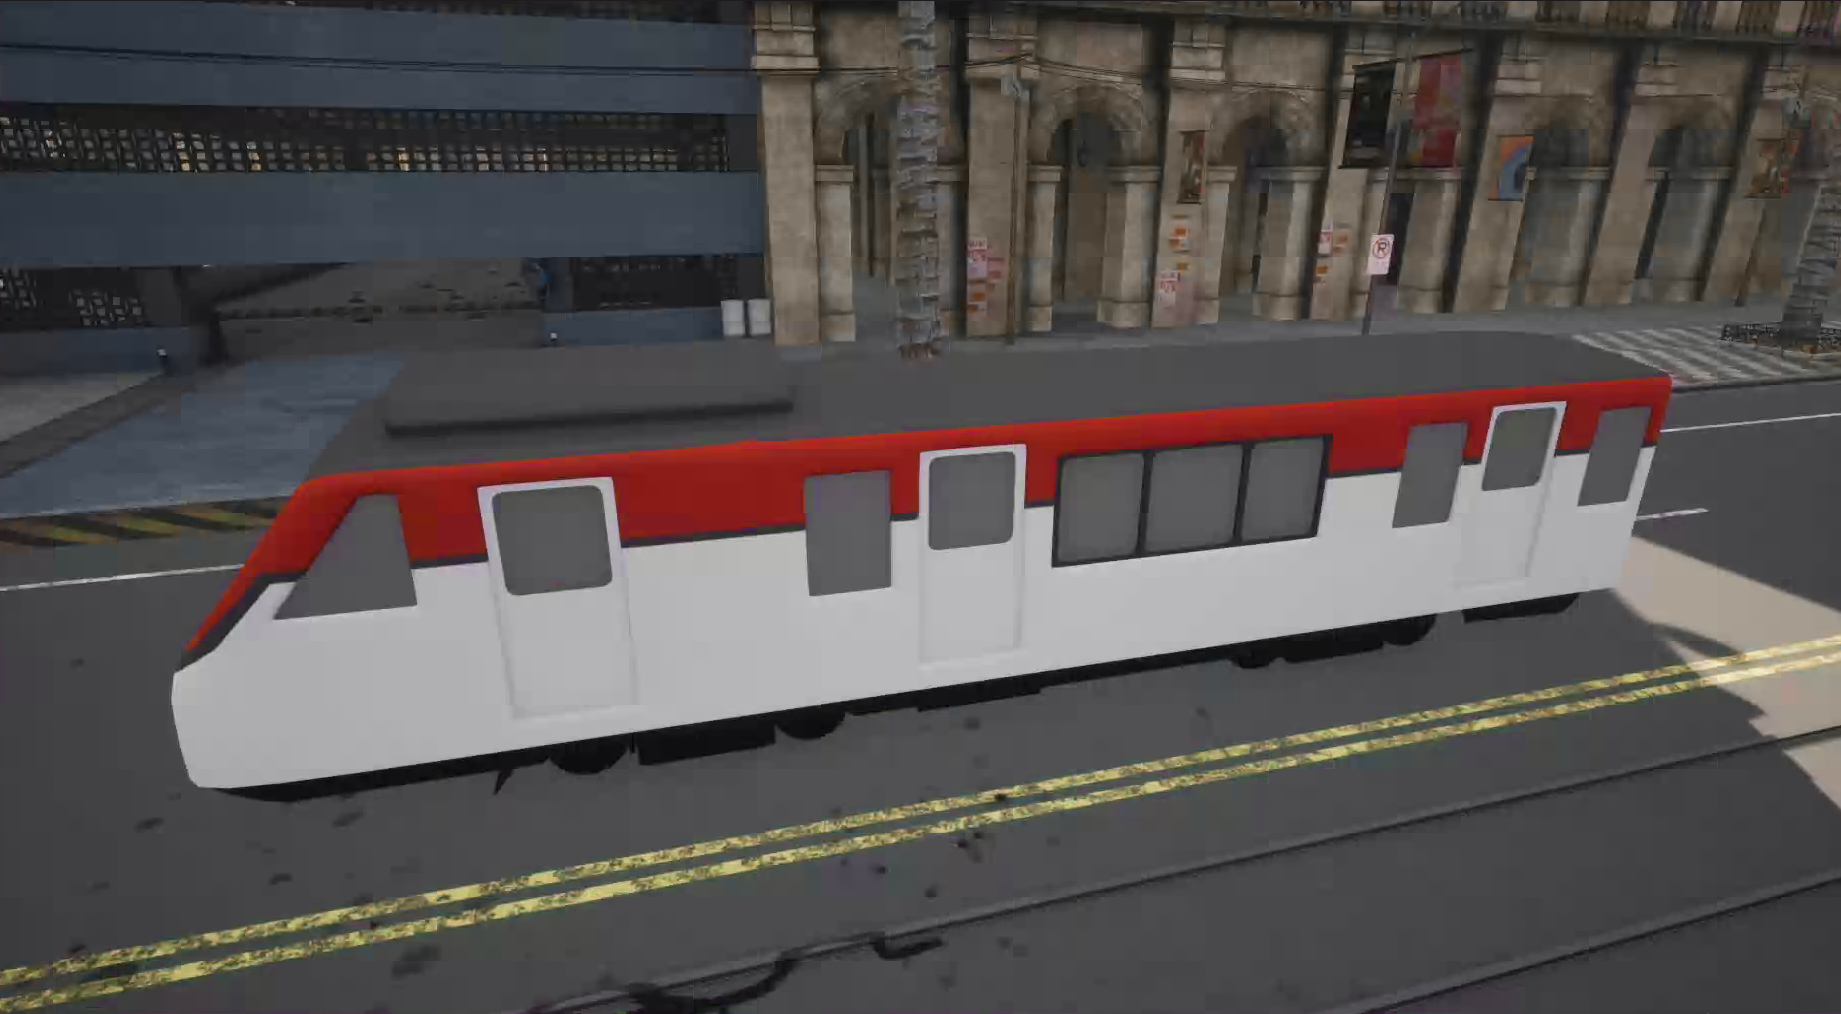
\includegraphics[width=0.6\textwidth]{resources/chapter-4/tram-carla.png}
    \caption{Implementasi trem dalam lingkungan simulasi}
    \label{fig:tram-carla}
\end{figure}

\begin{figure}[!h]
    \centering
    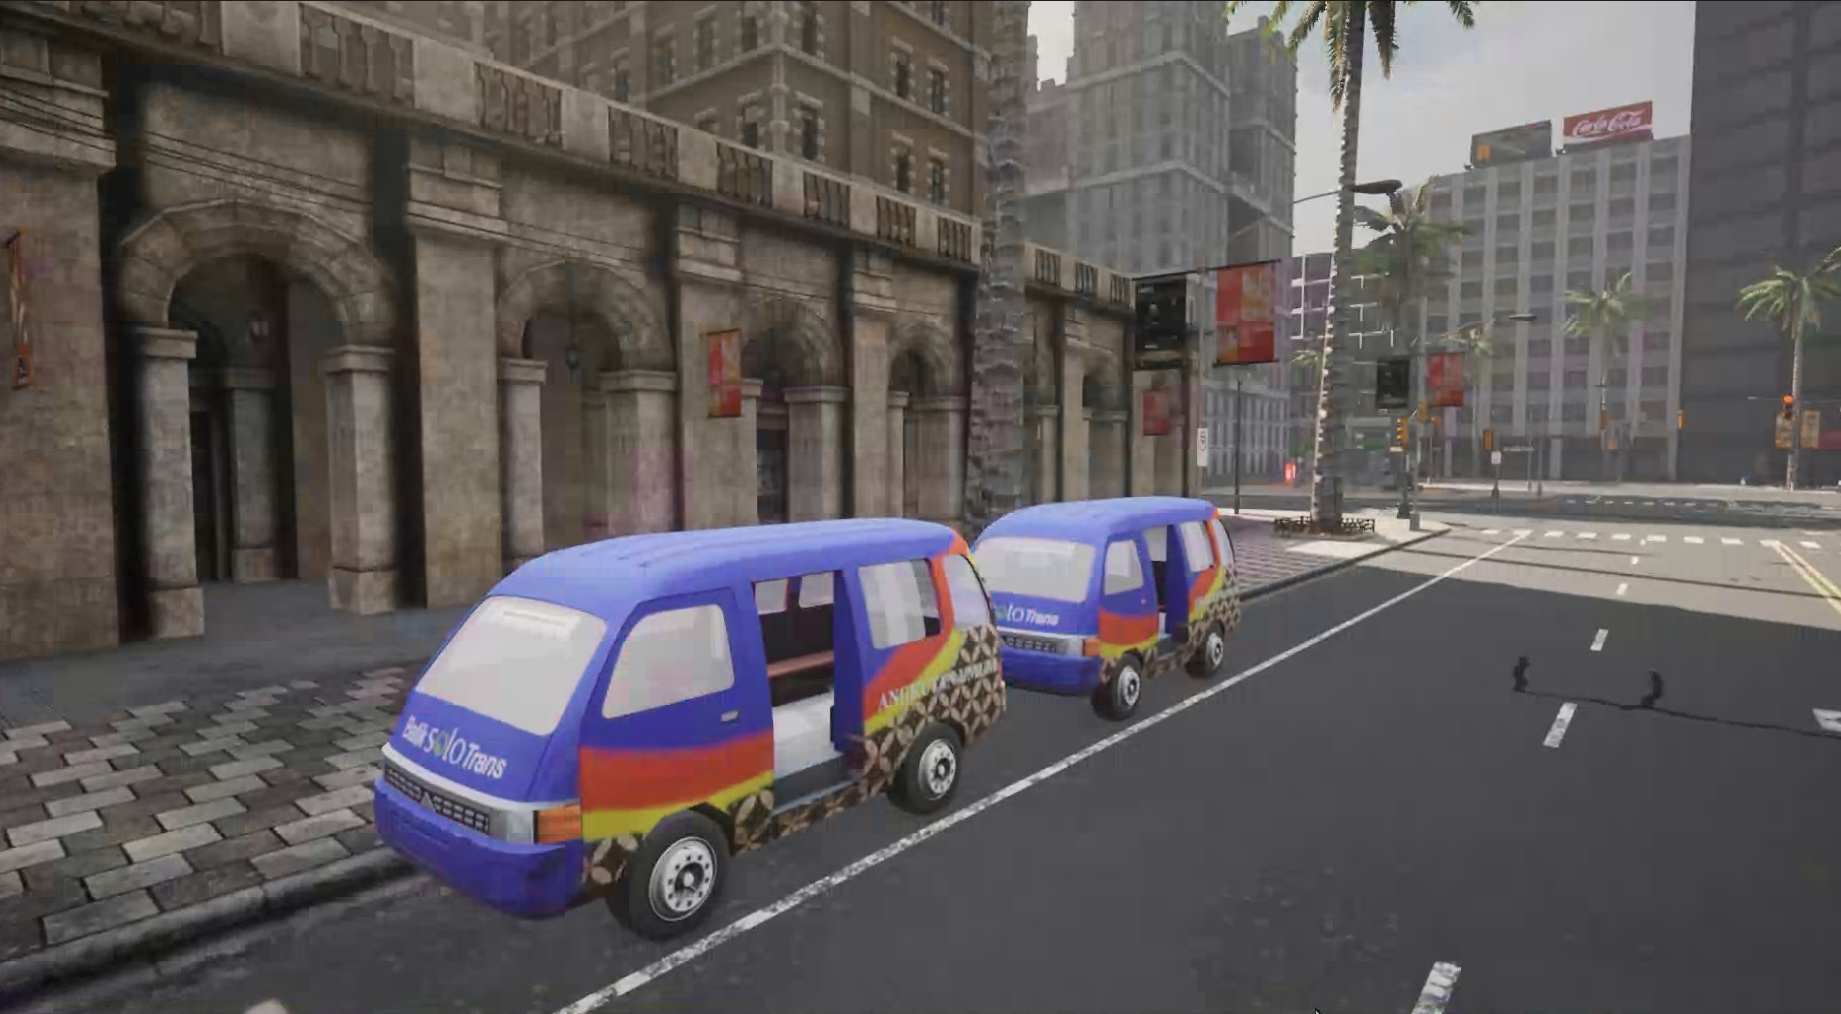
\includegraphics[width=0.6\textwidth]{resources/chapter-4/angkot.png}
    \caption{Implementasi angkot dalam lingkungan simulasi}
    \label{fig:angkot-carla}
\end{figure}

\section{Implementasi Lingkungan}

Penambahan aset model 3D ke dalam lingkungan simulasi dilakukan dengan membuat
folder baru pada direktori yang bersangkutan kemudian mengimpor aset model 3D ke
dalam folder tersebut. Cara menambahkan objek-objek statis ini adalah dengan
menarik objek dari impor dari \textit{Content Browser} ke dalam \textit{World
Outliner}. Setelah itu, dapat dilakukan penyesuaian skala, posisi, dan rotasi
aset pada \textit{World Outliner}. Penyesuaian lingkungan dapat dilakukan dengan
memilih dan mengaktifkan tingkat atau level objek yang ingin diubah.

% TODO: insert images, add directories, world levels, world outliner kah istilahnya?
% penyesuiannya lingkungan?

% TODO: benerin kata2nya jelek banget astaga

\subsection{Stasiun Madiun dan Stasiun Solokota}
Gambar \ref{fig:stasiun-madiun} menunjukkan implementasi model Stasiun Madiun
(lihat Gambar \ref{fig:stasiun-madiun-model}). Model stasiun kemudian
disesuaikan ukurannya dan diposisikan pada ... .

Gambar \ref{fig:stasiun-solokota} menunjukkan implementasi model Stasiun Solokota
(lihat Gambar \ref{fig:stasiun-solokota-model}). Model stasiun kemudian
disesuaikan ukurannya dan diposisikan pada ... .

% TODO: ..., + cara,  ke bab 3?

\begin{figure}[!h]
    \centering
    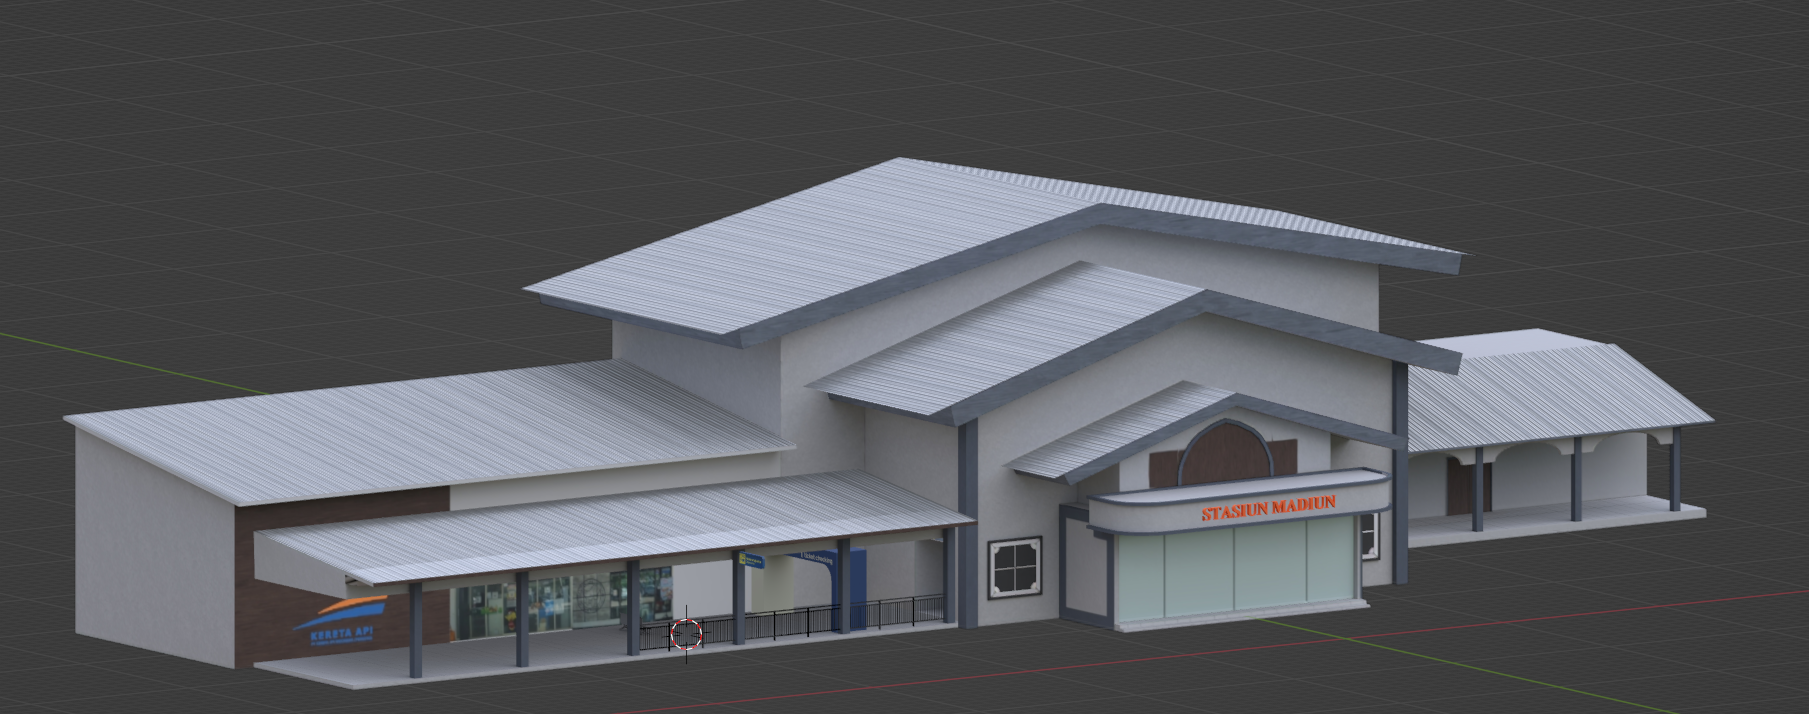
\includegraphics[width=0.6\textwidth]{resources/chapter-3-stasiun-madiun-model.png}
    \caption{Model Stasiun Madiun}
    \label{fig:stasiun-madiun-model}
\end{figure}

\begin{figure}[!h]
    \centering
    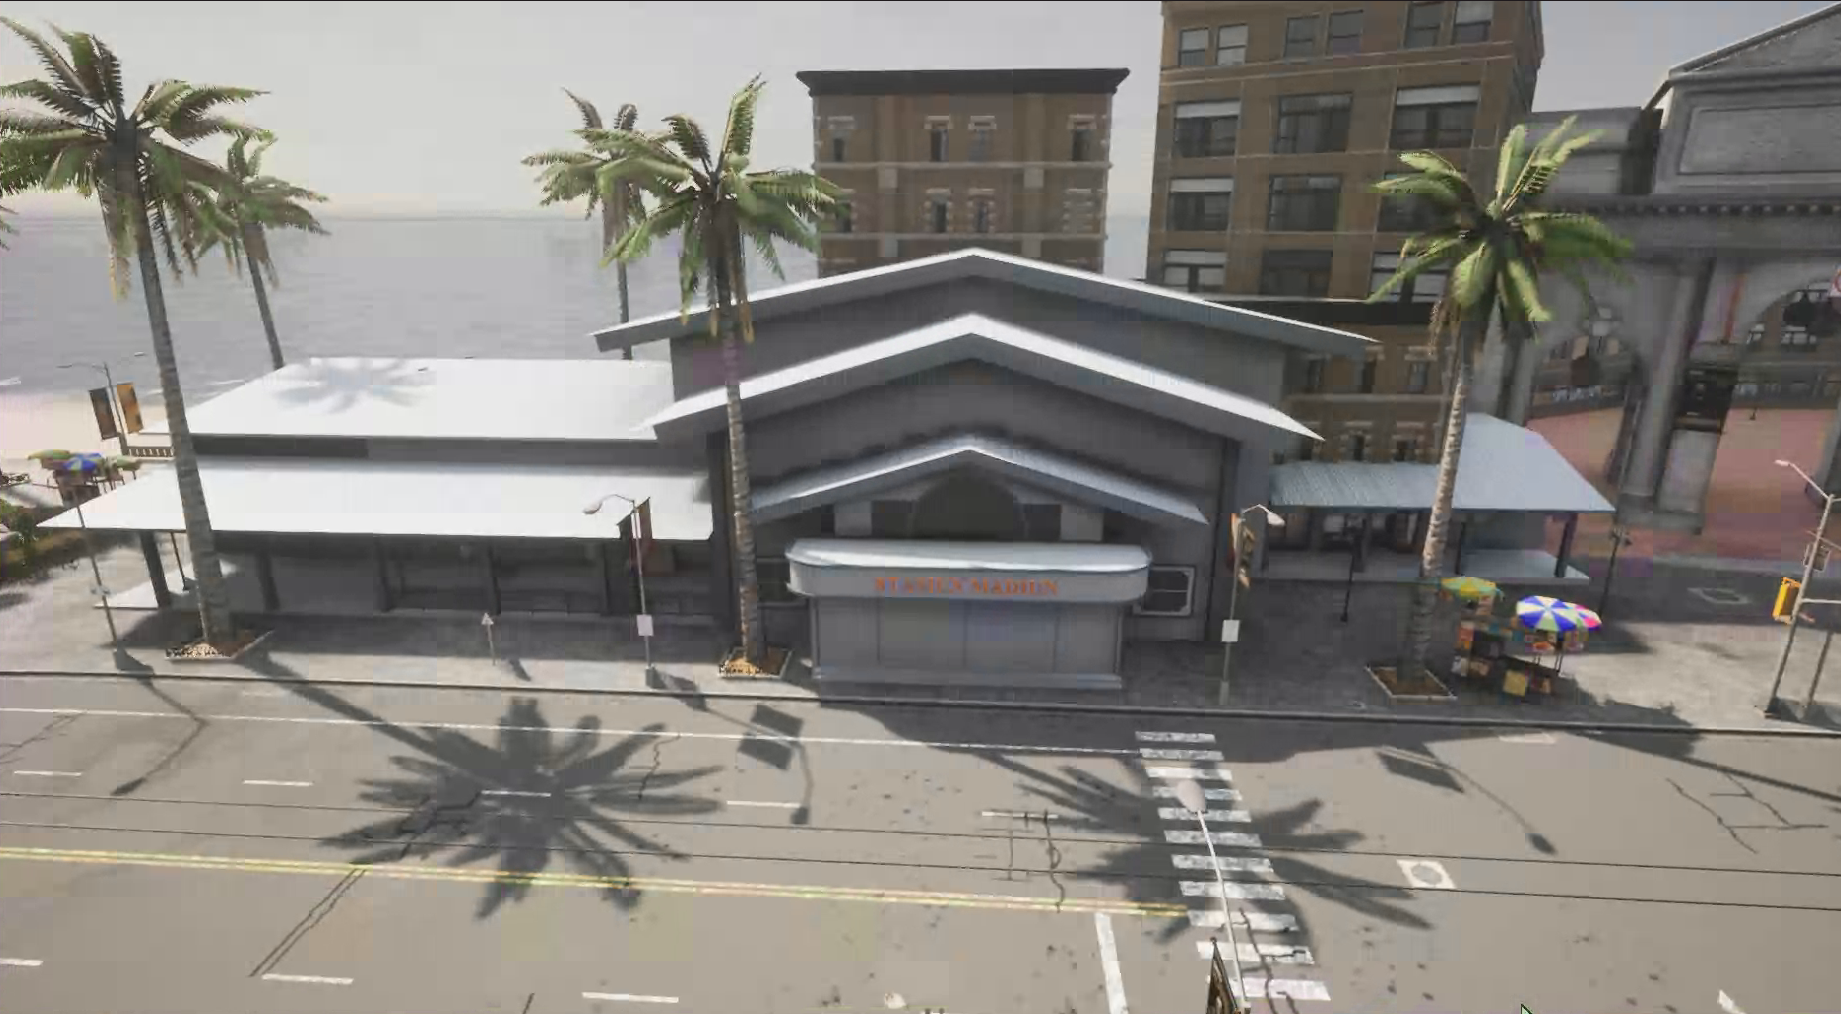
\includegraphics[width=0.6\textwidth]{resources/chapter-4/stasiun-madiun-carla.png}
    \caption{Implementasi stasiun Madiun dalam lingkungan simulasi}
    \label{fig:stasiun-madiun}
\end{figure}

\begin{figure}[!h]
    \centering
    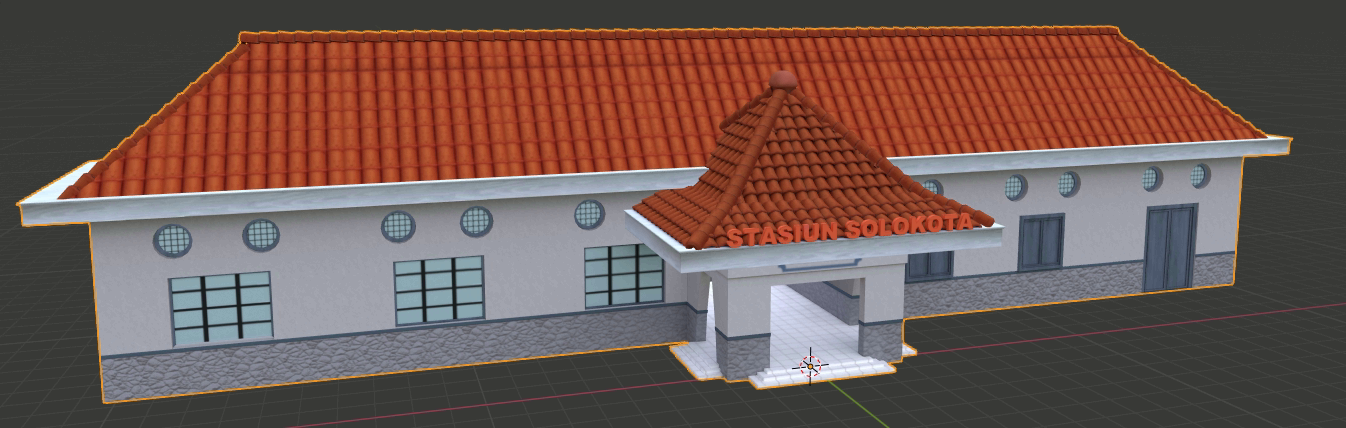
\includegraphics[width=0.6\textwidth]{resources/chapter-3-stasiun-solokota-model.png}
    \caption{Model Stasiun Solokota}
    \label{fig:stasiun-solokota-model}
\end{figure}

\begin{figure}[!h]
    \centering
    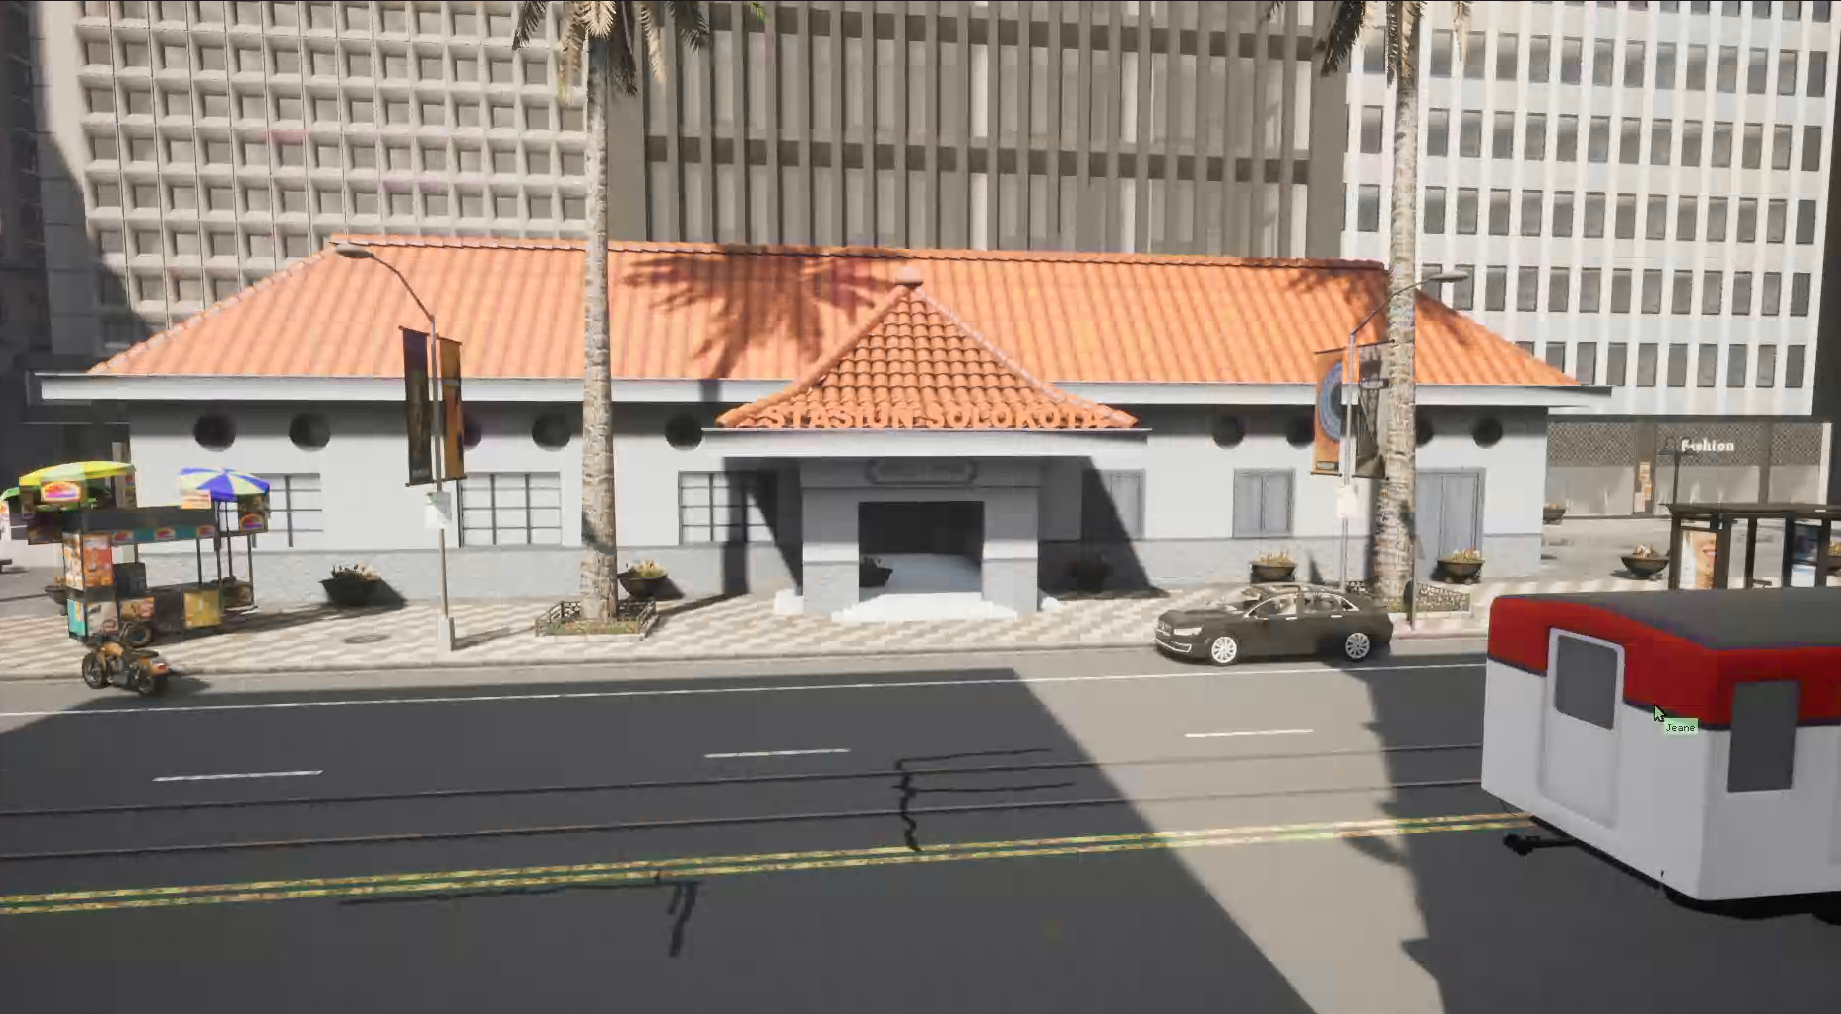
\includegraphics[width=0.6\textwidth]{resources/chapter-4/stasiun-solokota-carla.png}
    \caption{Implementasi stasiun Solokota dalam lingkungan simulasi}
    \label{fig:stasiun-solokota}
\end{figure}

\subsection{Rambu-rambu Lalu Lintas}

\begin{figure}[!h]
	\centering
	\subfloat[]{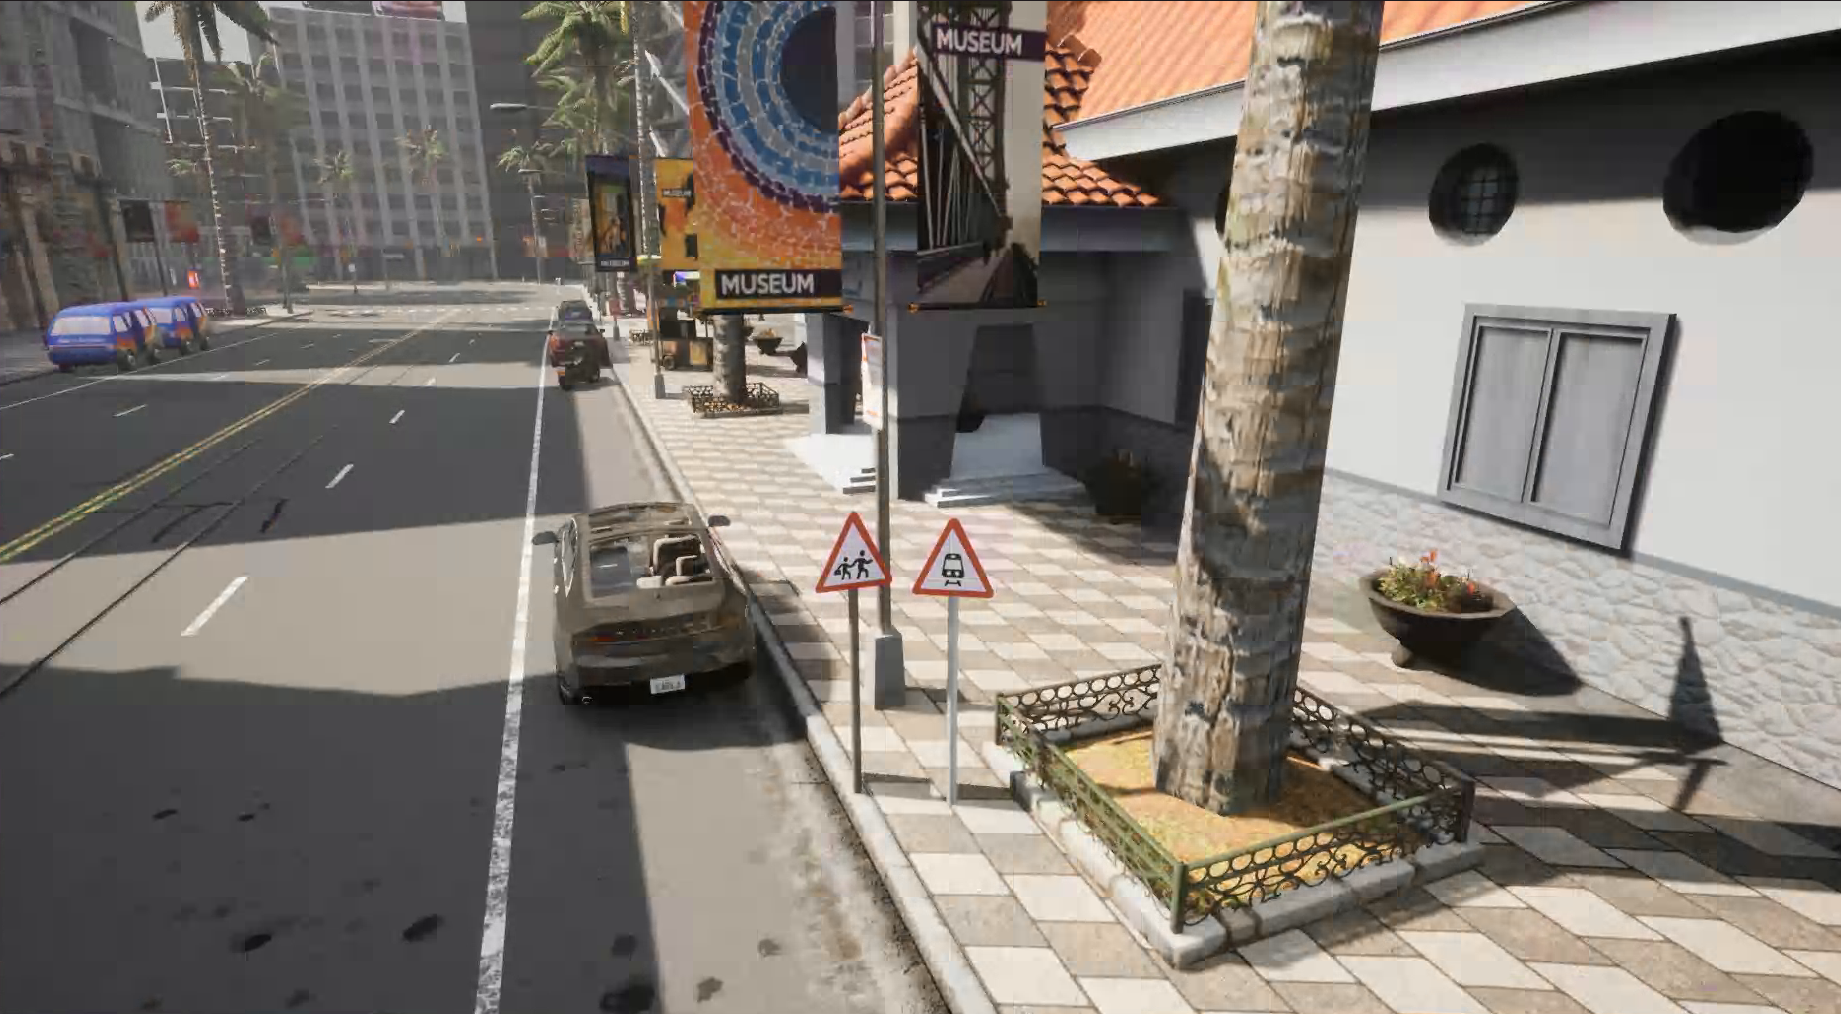
\includegraphics[width=0.45\textwidth]{resources/chapter-4/rambu-1.png}}
	\hfill
	\subfloat[]{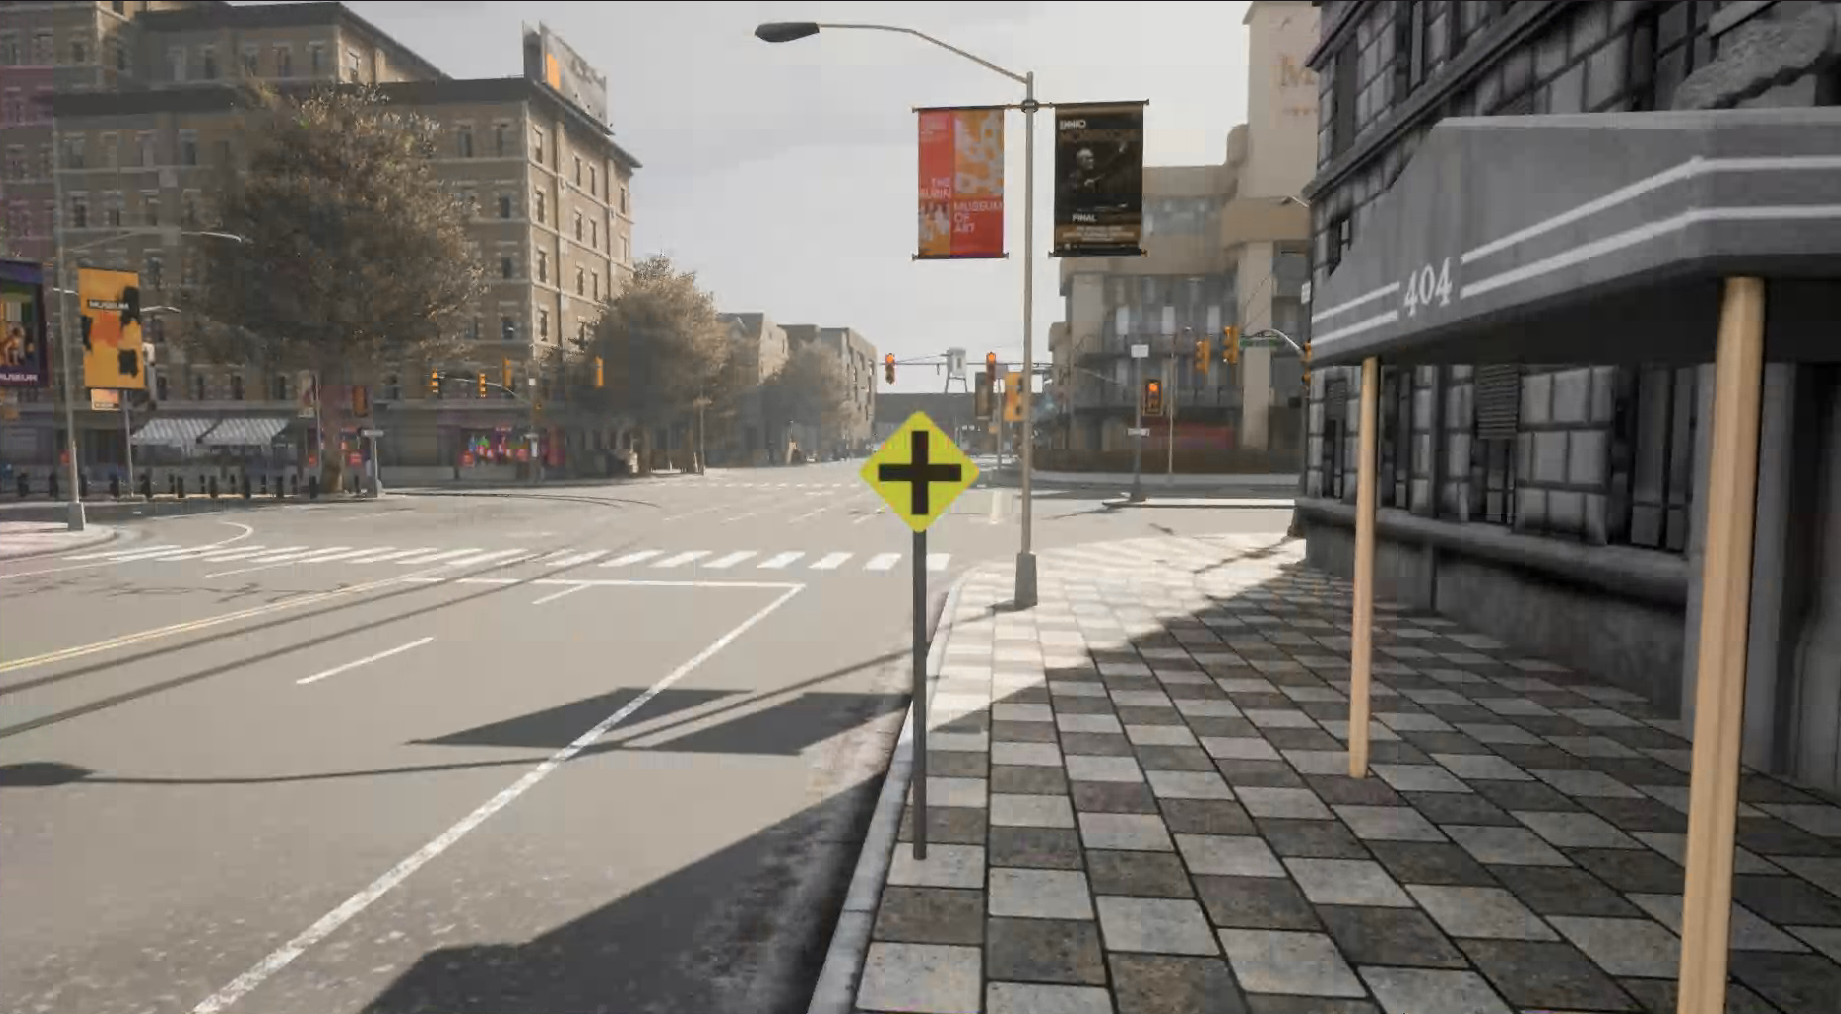
\includegraphics[width=0.45\textwidth]{resources/chapter-4/rambu-2.png}}
	\caption{Implementasi rambu-rambu lalu lintas dalam lingkungan simulasi}
	\label{fig:road-signs}
\end{figure}

\subsection{Rel}
% import mesh sebagai objek statis
% spline: butuh banyak edge/verts
% topview + stasiun

Gambar \ref{fig:rel} dan Gambar \ref{fig:rel-2} menunjukkan hasil implementasi rel.

% rel (lihat Gambar \ref{fig:rel-model}).

% \begin{figure}[!h]
%     \centering
%     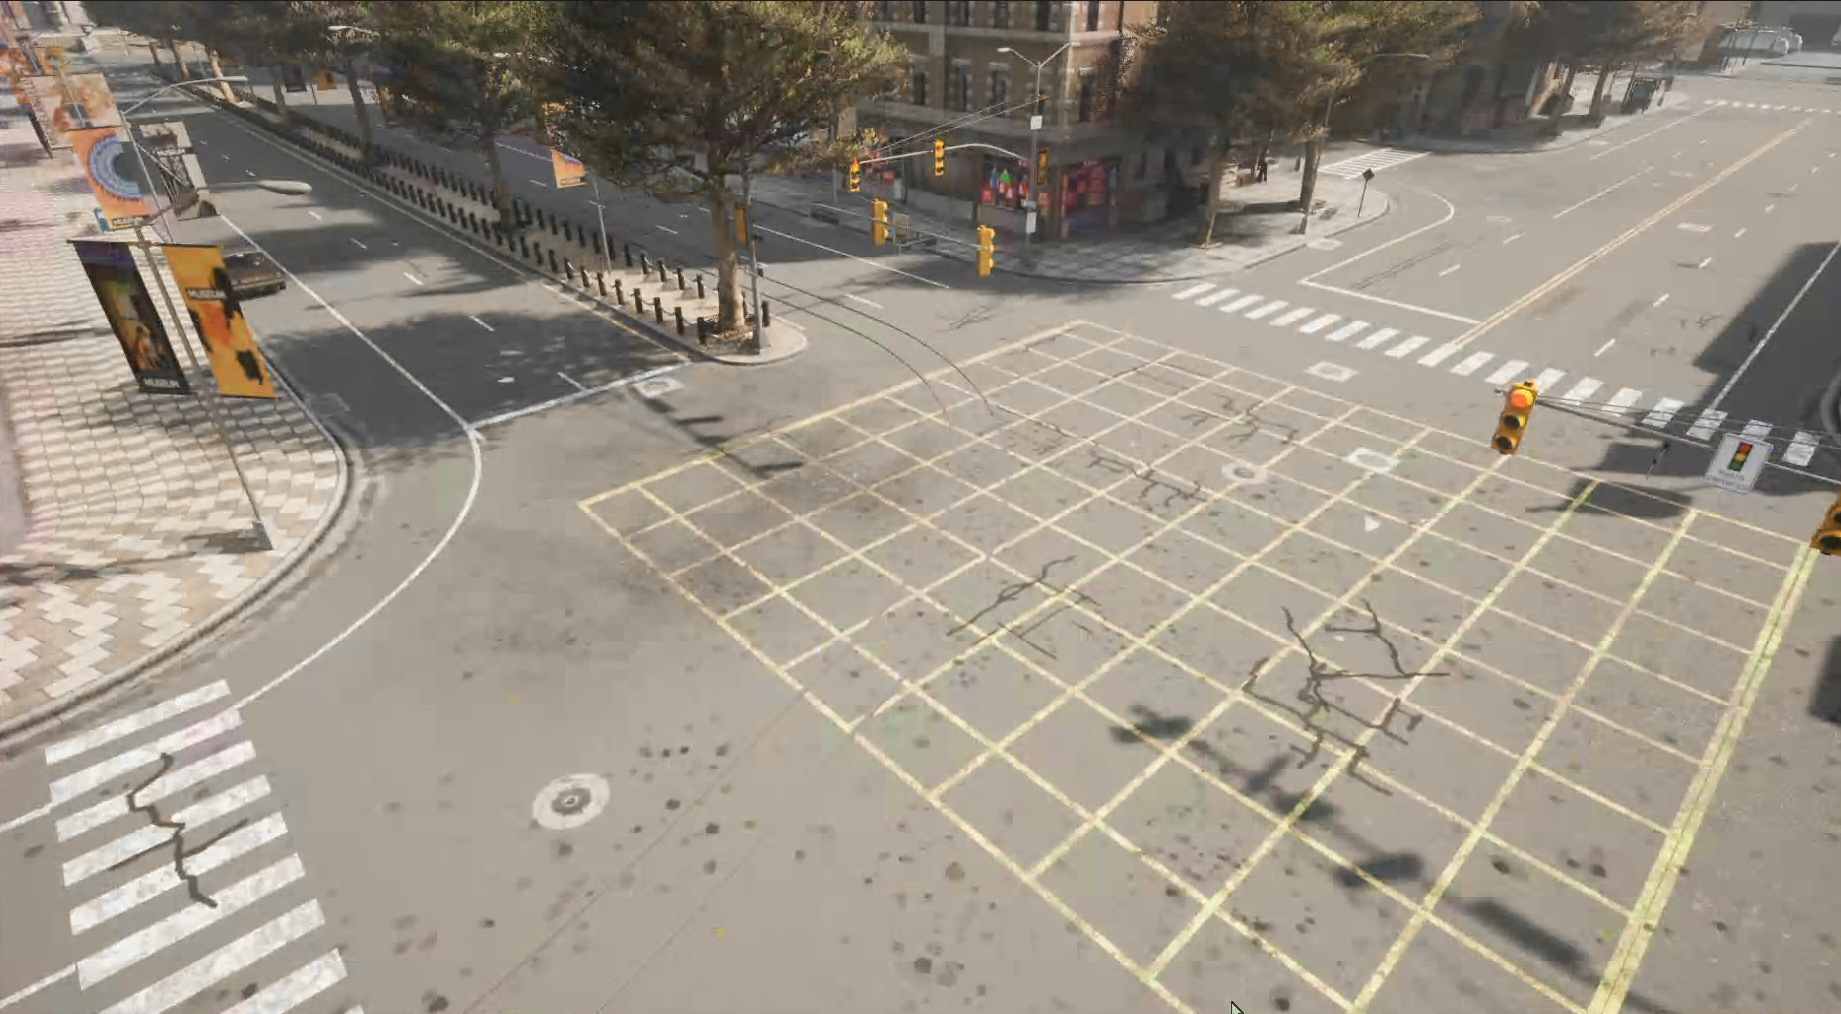
\includegraphics[width=0.6\textwidth]{resources/chapter-4/rel.png}
%     \caption{Implementasi rel dalam lingkungan simulasi}
%     \label{fig:rel-model}
% \end{figure}

\begin{figure}[!h]
    \centering
    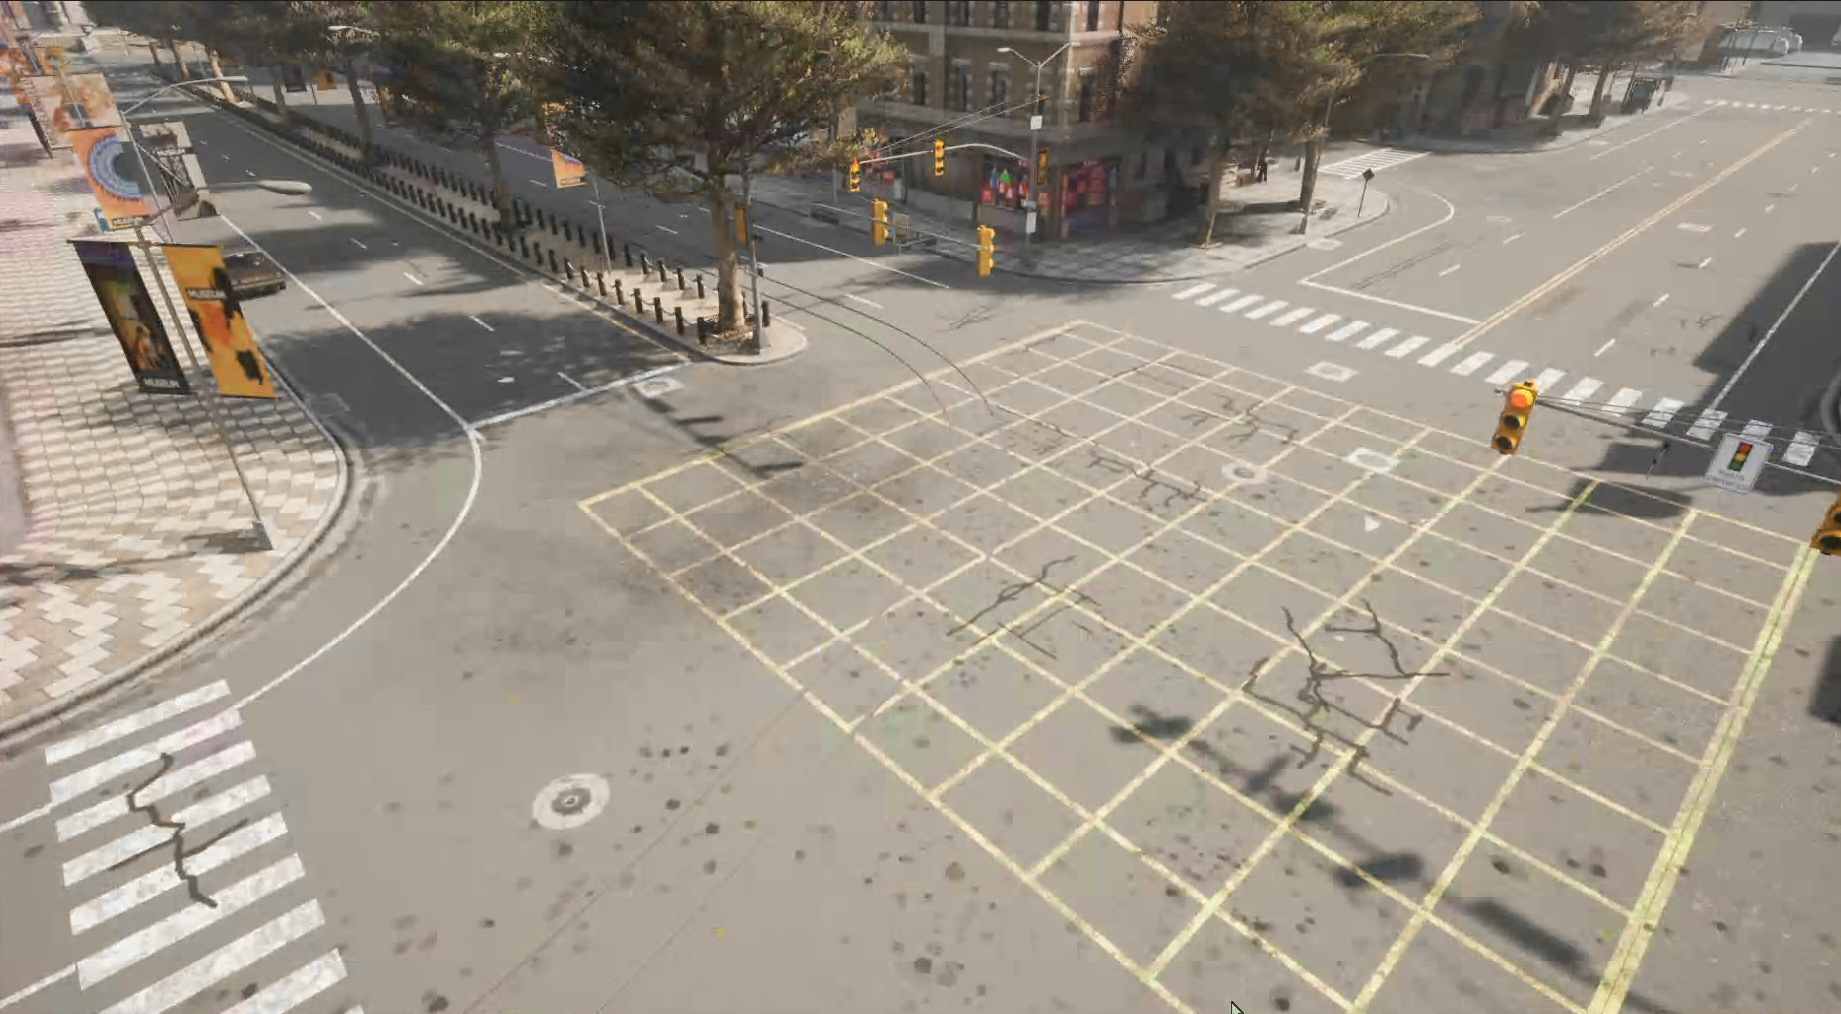
\includegraphics[width=0.6\textwidth]{resources/chapter-4/rel.png}
    \caption{Implementasi rel dalam lingkungan simulasi}
    \label{fig:rel}
\end{figure}

\begin{figure}[!h]
    \centering
    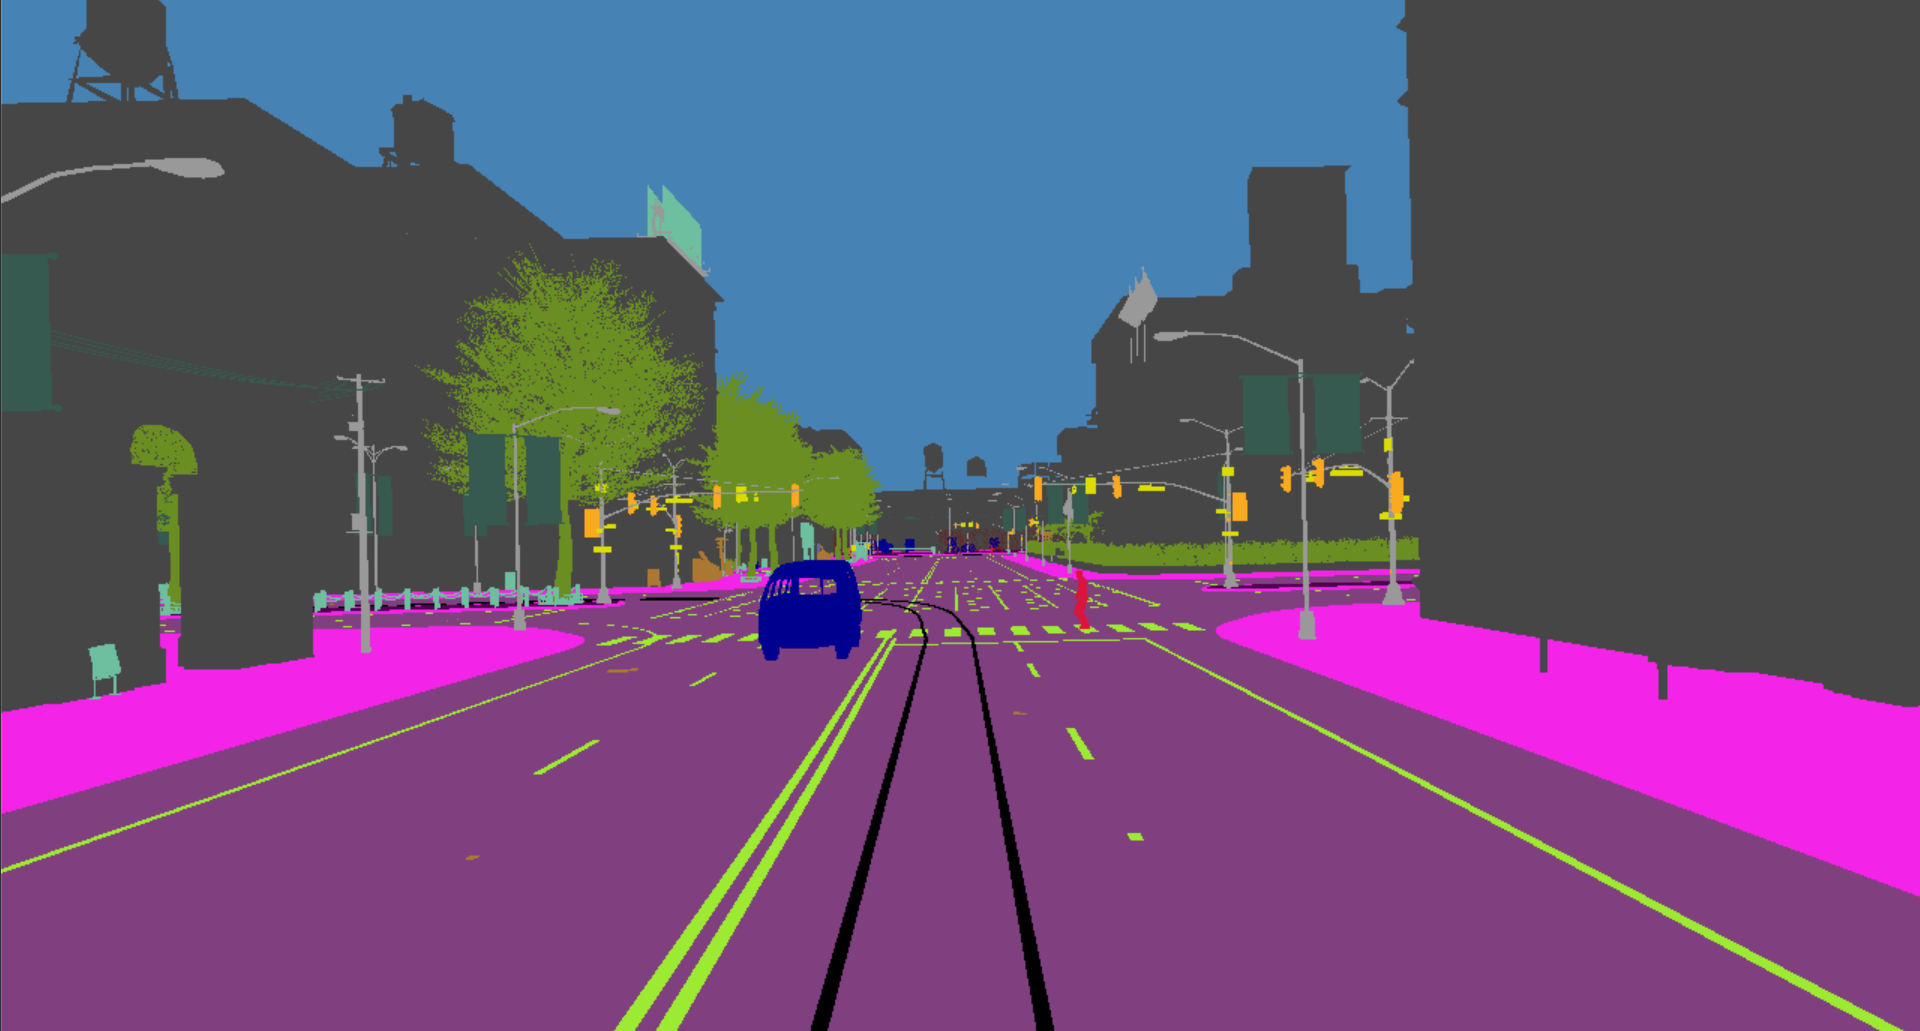
\includegraphics[width=0.6\textwidth]{resources/chapter-4/rel-segmentation-camera.png}
    \caption{Implementasi rel dalam lingkungan simulasi (tampilan segmentasi semantik)}
    \label{fig:rel-2}
\end{figure}

\section{Validasi}

\subsection{Tujuan Validasi}

Tujuan validasi adalah untuk memastikan bahwa objek2 berperilaku normal (seperti
aslinya) dan stabil saat simulasi berjalan.

% TODO:

\subsection{Hasil Validasi}
% manual + generate

\section{Distribusi Hasil Implementasi}

\section{Evaluasi}
% kendaraan roda 2 dan 3 berhasil diimplementasikan namun tidak stabil
% ? tidak diperlukan perta
% tidak diperlukan data OpenDRIVE untuk traffic signs, karena:
% - tidak dibutuhkan
% - dari sisi trem, hanya butuh secara visual saja
% - dari sisi kendaraan lain (untuk autopilot), tidak dibutuhkan juga, mostly cuman penanda ada ini

% \chapter{Penutup}

\section{Kesimpulan}
\blindtext

\section{Saran}
\blindtext
%----------------------------------------------------------------%

% Daftar pustaka
\printbibliography
% \blankpage

% Setting judul lampiran
\titlespacing*{\chapter}{0pt}{0pt}{0pt}
\titlespacing*{\section}{0pt}{0pt}{*1}

% Setting judul anak lampiran
\titleformat*{\section}{\bfseries}

% Index
\appendix
% \chapter{Rancangan Sistem}\label{appendix-arsitektur-baru}
% TODO: find a better way to set counter
\setcounter{section}{1}
\begin{figure}[ht]
	\centering
	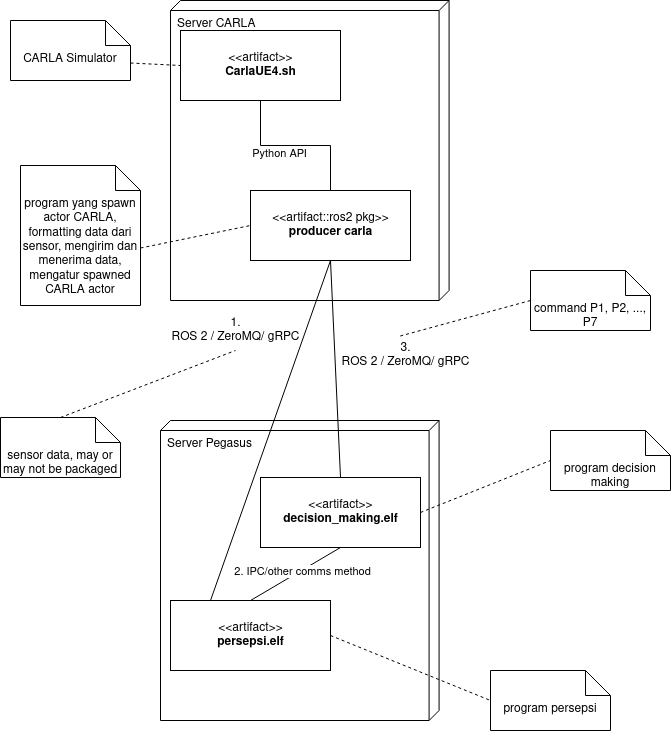
\includegraphics[width=1.0\textwidth]{resources/appendix-1-deployment diagram.png}
	\caption{Rancangan Sistem Simulasi}
\end{figure}
% \chapter{Contoh Judul Lampiran}
Here is my appendix content...

\end{document}
